\documentclass[a4paper,fleqn]{cas-dc}

\usepackage[numbers,sort,compress]{natbib}
% \usepackage{graphics}
\usepackage{subcaption}
\usepackage[section]{placeins}
\usepackage{textcomp}
\usepackage{pgfplots}
\pgfplotsset{width=10cm,compat=1.9}
% \usepackage[table]{xcolor}
%%%Author macros
\def\tsc#1{\csdef{#1}{\textsc{\lowercase{#1}}\xspace}}
\tsc{WGM}
\tsc{QE}
\tsc{EP}
\tsc{PMS}
\tsc{BEC}
\tsc{DE}
%%%

% \usepackage{tables}
\usepackage{diagbox}
\usepackage{rotating}
\usepackage{tabu}                    
\usepackage{multirow}                 
\usepackage{multicol}                 
\usepackage{multirow}                
\usepackage{float}                   
\usepackage{makecell}                 
\usepackage{booktabs}                 
\begin{document}
\sloppy
\let\WriteBookmarks\relax
\def\floatpagepagefraction{1}
\def\textpagefraction{.001}

% Short title
\shorttitle{Rapid diagnosis technology for acute heart failure based on auscultation}

% Short author
\shortauthors{Hui et~al.}  

% Main title of the paper
\title [mode = title]{Rapid diagnosis technology for acute heart failure based on auscultation}                      

% Author
\author[1]{Hui Yu}
\author[1]{Zhaoyu Qiu}[orcid=0000-0002-7728-7367]
\author[2]{Zhigang Li}
\author[1]{Jinglai Sun}
\author[1]{Guangpu Wang}
\author[1]{Jing Zhao}\ead{zhaojing_zj@tju.edu.cn}
\cormark[1]
\author[1]{Shuo Wang}\ead{ws111@tju.edu.cn}
\cormark[1]
%\author[1]{Jing Zhao}[ ]
%\author[1]{Hui Yu}[]
%\author[2]{Gangde Li}[]

\credit{Conceptualization, Methodology, Writing original draft}

% \cortext[cor1]{These authors contributed equally to this work.}
\cortext[cor1]{Corresponding author}
% Address/affiliation
\affiliation[1]{organization={Department of Biomedical Engineering},
                addressline={Tianjin University}, 
                city={Tianjin},
                postcode={300072},
                country={China}}


\affiliation[2]{organization={Department of Emergency Medicine},
                addressline={Tianjin 4TH Centre Hospital},
                city={Tianjin},
               postcode={300142},
               country={China}}

\begin{abstract}
    \noindent Background and Objectives: Acute Heart Failure (AHF) results in over 26 million hospital admissions worldwide annually, posing a significant global health concern. Currently, AHF diagnosis relies on biochemical markers and echocardiography, which take more than 20 minutes. Auscultation, a quick and non-invasive clinical practice, is used alongside the gold standard. To address the need for rapid clinical AHF diagnosis, this paper presents a model for feature extraction and diagnosis using short heart sound signals.\\
    \noindent Methods: Discrete wavelet transform was applied for heart sound denoising, and Mel Frequency Cepstrum Coefficients were used for feature extraction. A new DenseHF-Net is proposed for diagnosing heart failure. Additionally, a feature fusion method is introduced for multi-region fusion auscultation, including mitral, aortic, and pulmonic valves, along with an ensemble method for long auscultation in the mitral valve region. \\
    \noindent Results: An auscultation dataset containing 2999 recordings, each with rich annotations, has been established. The proposed wavelet denoising algorithm achieved a signal-to-noise ratio of 7.8 dB. For multi-region fusion auscultation using DenseHF-Net, the average accuracy reached 99.25\%. For mitral valve ensemble auscultation, the average accuracy was 92.60\%.\\
    \noindent Conclusions: The proposed method enables rapid auscultation for AHF, providing accurate results based on a 3-second auscultation recording. While multi-region fusion auscultation achieves high accuracy, mitral valve ensemble auscultation offers a good balance between efficiency and accuracy. This research has the potential to be applied in cardiac auscultation tools for mobile phones, cloud-based systems, or electronic gloves. Data and codes are accessible on \href{https://github.com/qiuzhaoyu/AHF-Rapid-Diagnosis}{https://github.com/qiuzhaoyu/AHF-Rapid-Diagnosis}.\\
    \end{abstract}
    

% Research highlights
\begin{highlights}
\item An auscultation dataset has been established, containing 2999  recordings from heart failure patients, each with rich annotations, and are publicly accessible on \href{https://github.com/qiuzhaoyu/AHF-Rapid-Diagnosis/Database}{https://github.com/qiuzhaoyu/AHF-Rapid-Diagnosis/Database}.
% \item A wavelet denoising algorithm and a lightweight DenseHF-Net have been developed for short-duration auscultation, aiming at rapid diagnosis of acute heart failure.
% \item We have introduced two auscultation strategies: multi-region fusion auscultation and mitral valve auscultation. Multi-region fusion auscultation is designed for monitoring scenes, while mitral valve auscultation is designed for rapid diagnosis in cases of heart failure emergencies.
\end{highlights}

\begin{keywords}
\sep Heart Sound Signal\sep Acute Heart Failure\sep Mel Frequency Cepstrum Coefficient\sep Lightweight Deep Learning Model
\end{keywords}

\maketitle



% \section{Introduction}\label{sec:introduction}
\subsection{Background}
Cardiovascular disease (CVD), including heart failure (HF) and stroke, has become the leading cause of death and disability worldwide \cite{virani2020heart,roth2020global,mensah2019global,boorsma2020congestion}. The rising age-standardized rate of CVD is especially evident in almost all non-high-income countries \cite{roth2020global}. Heart failure, particularly in its acute form (AHF), represents a critical stage in CVD, characterized by the heart's impaired ability to contract and stretch. AHF is a leading cause of emergency hospital admissions, especially among the elderly population \cite{sinnenberg2020acute,arrigo2020acute}. It accounts for over 26 million hospital admissions annually, with a mortality rate ranging from 20-30\% \cite{chapman2019clinical}. In managing AHF, emergency procedures like ambulance response and door-to-balloon time are crucial, as shortening these can significantly reduce patient mortality and morbidity \cite{victor2012door,fan2021effects}. For instance, in myocardial infarction—a common cause of AHF—reducing ambulance response time by 15.3 minutes and door-to-balloon time by 36 minutes has been shown to decrease hospital stays by 6.3 days, lower mortality by 12.33\%, and reduce rehospitalization rates by 19.69\% \cite{fan2021effects}. Consequently, optimizing these procedures, particularly by shortening door-to-balloon time and conducting rapid diagnostics such as auscultation during ambulance transport, can greatly enhance survival rates in AHF patients. However, traditional AHF diagnostic methods, including auscultation, need further optimization. While auscultation is a key rapid diagnostic tool, its effectiveness in ambulance scenarios requires additional quantitative evaluation to ensure it meets the urgent demands of modern emergency care.

Traditional AHF diagnosis relies heavily on clinical biochemical trials, and there is a significant lack of convenient and accurate diagnostic methods, particularly for the 20\% of patients with no history of chronic heart failure (CHF). According to the European Society of Cardiology's AHF First Aid Guidelines, the diagnostic criteria for AHF encompass clinical evaluation, electrocardiogram (ECG), chest x-ray, imaging techniques, laboratory tests, and echocardiography \cite{nieminen2005task}. Diagnosis typically hinges on the patient's history and physical examination, supplemented by physical tests such as ECG, echocardiography, and biochemical markers like brain natriuretic peptide (BNP) and NT-proBNP. However, current methods are time-consuming; for example, mainstream NT-proBNP and BNP biochemical detection equipment reports waiting times of 9-16 minutes for BNP results and 11-21 minutes for NT-proBNP results \cite{lewis2020bnp}. Additionally, echocardiography, which provides crucial information on the ejection fraction for preoperative evaluation of AHF, requires about 20-30 minutes for a single examination, including approximately five minutes for equipment setup \cite{menon2022echocardiography}. These time requirements highlight the need for more rapid and accessible diagnostic tools, especially in emergency settings where timely decision-making is critical.

Auscultation, as part of the clinical evaluation, is an effective means of diagnosing heart failure and is recommended by the European Society of Cardiology as a class-1 method \cite{nieminen2005task}. Heart sounds are produced by the mechanical motion of the heart's dynamic system, comprising various mechanical vibrations caused by blood movement within the cardiovascular system. These heart sounds contain a wealth of information regarding the physiology of the cardiovascular system and serve as a crucial auditory representation of the heart's contractile and stretch functions \cite{johnston2007third,wynne2001clinical,boorsma2020congestion}. Normal heart sounds consist of four distinct tones, known as the first heart sound (S1), second heart sound (S2), third heart sound (S3), and fourth heart sound (S4), occurring in sequence during the cardiac cycle. The mitral valve, aortic valve, pulmonary valve, and tricuspid valve are the four most commonly used auscultation areas. The tricuspid valve area, in particular, is crucial for detecting right heart failure. Unlike ECG, which records electrical activity, heart sounds reflect the ventricle's ability to pump blood, providing potentially richer pathological information within a single cardiac cycle. Abnormal heart sounds generally exhibit more background noise, greater fluctuations in S1 amplitude, and more high-frequency details compared to normal heart sounds, making auscultation a valuable tool for early detection of heart dysfunction.
\subsection{Related works}
The current research on digital auscultation technology encompasses aspects such as datasets, signal processing, and diagnostic models.

In terms of datasets, the most commonly utilized dataset is the one established by PhysioNet for the Heart Sound Classification Challenge in 2016 \cite{clifford2016classification}, including 665 abnormal heart sounds and 2575 normal heart sounds. Yaseen et al. \cite{son2018classification} provided a five-classification dataset of Aortic Stenosis (AS), Mitral Regurgitation (MR), Mitral Stenosis (MS), Mitral Valve Prolapse (MVP) and Normal (N), with 200 cases of each type. Nonetheless, for the development of algorithms aimed at diagnosing a particular medical condition, the current dataset may exhibit limitations in terms of annotation richness. Therefore, to develop rapid diagnostic models for AHF, additional efforts are needed to refine the data and standardize inclusion criteria.

In the realm of pre-processing and feature extraction for heart sounds, various techniques have been developed to analyze these signals effectively. For instance, Vepa's research \cite{vepa2009classification} utilized Short-Time Fourier Transform (STFT) and Discrete Wavelet Transform (DWT) to process heart sound signals. Wu et al. \cite{wu2010hidden} extracted Mel-Frequency Cepstral Coefficients (MFCC) components of heart sound signals based on the hidden Markov model (HMM). Techniques such as MFCC-based feature extraction have proven to be highly successful and widely adopted in heart sound processing. While there are classification algorithms capable of handling short-duration phonocardiogram (PCG) segments, often as short as 2 seconds with majority voting for final output, many existing methods are optimized for longer signal durations, which may not always be ideal for the rapid diagnosis required in acute heart failure (AHF) scenarios. This highlights the need for further optimization of these techniques to ensure they are suitable for the time-sensitive nature of AHF diagnosis.

In terms of diagnostic models, Rubin \cite{rubin2016classifying} used a convolutional neural network (CNN) for heart sound signal classification by time-frequency characteristics. Arora et al. \cite{arora2021transfer} performed transfer learning of heart sound signals based on VIZ, MobileNet, Xception, VGG, ResNet, DenseNet and Inception. Scholars such as Li and Shuvo \cite{li2021lightweight,shuvo2021cardioxnet} have developed end-to-end lightweight neural networks for clinical mobile devices. The established models are too large in size for rapid diagnosis of AHF. Therefore, we have developed lightweight models and introduced different auscultation strategies for various clinical scenarios.

To address the challenges of signal processing and diagnostic model in AHF auscultation, our main contributions are:

\begin{itemize}
\item  An auscultation dataset has been established, containing 2999  recordings from heart failure patients, aiming at addressing the challenges in heart failure auscultation. This dataset encompasses comprehensive information, including diagnostic results, collection area annotations, medical history records, and annotations related to BNP and NT-proBNP. Additionally, this dataset has undergone a rigorous ethical review process and is publicly accessible on  \href{https://github.com/qiuzhaoyu/AHF-Rapid-Diagnosis}{https://github.com/qiuzhaoyu/AHF-Rapid-Diagnosis}.
\item A wavelet denoising algorithm and a lightweight DenseHF-Net have been developed for short-duration auscultation signals, aiming at rapid diagnosis of acute heart failure. The denoising algorithm proposed in this paper has improved the average signal-to-noise ratio to 7.8 dB. DenseHF-Net has only 0.33M parameters and is easily ported to low-computation scenarios such as mobile terminals. 
\item We have introduced two auscultation strategies: multi-region fusion auscultation and mitral valve auscultation. Multi-region fusion auscultation is designed for scenarios where long-time auscultation is possible, such as monitoring situations. It utilizes the three most crucial regions, namely, the mitral valve region, aortic valve region, and pulmonic valve region. On the other hand, mitral valve auscultation is specifically designed for rapid diagnosis in cases of heart failure emergencies, focusing solely on the mitral valve auscultation region. It completes the diagnosis within 15 seconds with an accuracy of 92.60\%.
\end{itemize}

% The remainder of this paper is arranged as follows:
% Paragraph.\ref{Materials and Methods} describes data denoising, feature extraction and models building. Paragraph.\ref{Results} describes the results of Paragraph.\ref{Materials and Methods}. Paragraph.\ref{Discussion} discusses the experimental results and compares them with other research. Paragraph.\ref{Conclusion} summarises the results and shortcomings of this paper, and suggests future research.
% \section{Materials and Methods}\label{Materials and Methods}
\begin{figure*}[htbp]
    \centering
    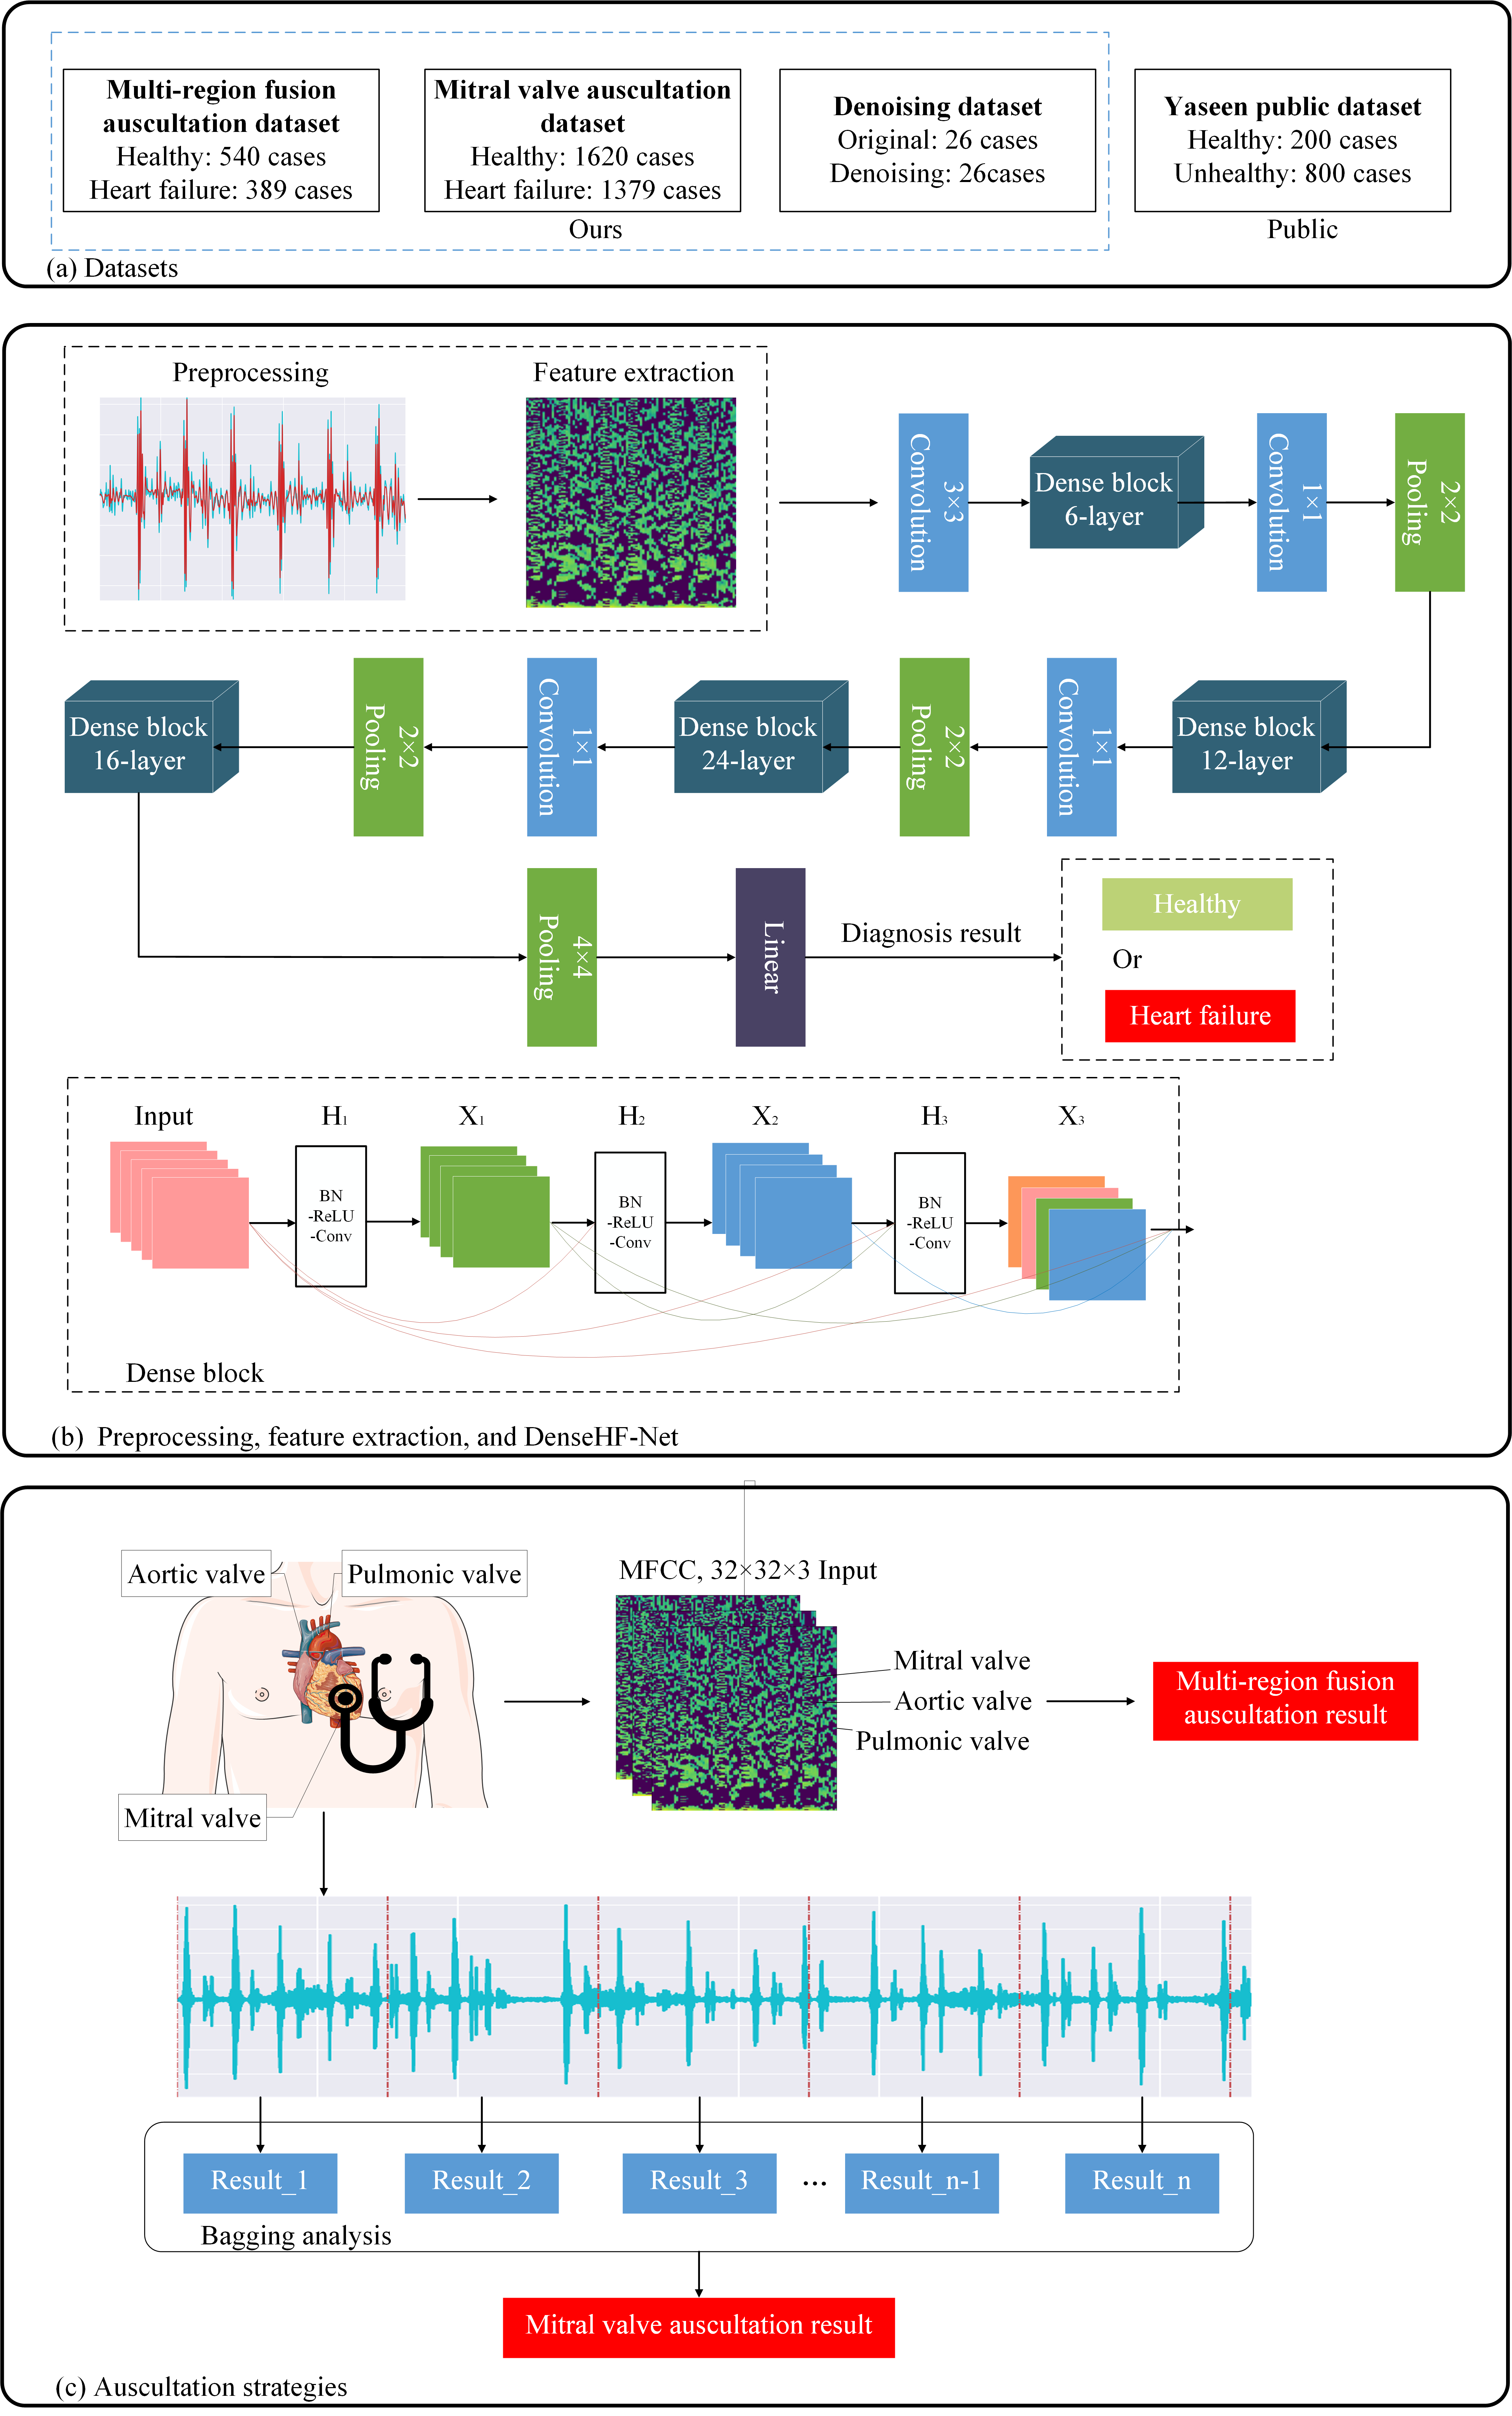
\includegraphics[width=0.77\linewidth]{figs/methods/all.png}
    \caption{\textbf{Methodology of the proposed work.} (\textbf{a}) A dataset was built in this paper, including two HF diagnostic subsets, a denoising subset, and a public subset. (\textbf{b}) The layered architecture of the proposed DenseHF-Net contains four Dense blocks. (\textbf{c}) Multi-region fusion auscultation and mitral valve auscultation.}
	\label{FIG:Methodology}
\end{figure*}
Fig. \ref{FIG:Methodology} illustrates the methodology employed in this paper. Firstly, in order to address the data scarcity issue in the development of AHF diagnostic models, we have created several datasets. We create a multi-region fusion auscultation dataset, containing 540 healthy cases and 389 heart failure cases. Each case includes three audio recordings corresponding to the mitral valve, aortic valve, and pulmonic valve. Additionally, a mitral valve auscultation dataset is established, containing 1620 healthy cases and 1379 heart failure cases, with each recording lasting between three to five seconds.

Next, in response to the signal processing and lightweight requirements for rapid AHF diagnosis, we have developed a wavelet denoising algorithm and a lightweight DenseHF-Net. We developed and implemented a wavelet denoising algorithm specifically designed for short-duration heart sound signals, effectively reducing noise. Subsequently, we employ the MFCC algorithm to extract one-dimensional sound signals into two-dimensional image features. Finally, a DenseHF-Net is used to train on the MFCC features.

This paper introduces two distinct auscultation strategies. 1. Multi-region fusion auscultation is designed for
scenarios where long-time auscultation is possible, using the fusion characteristics of the mitral valve, aortic valve, and pulmonic valve as input features. 2. Mitral valve auscultation is specifically
designed for AHF rapid diagnosis in cases of ambulances. In the case of mitral valve auscultation lasting more than 10 seconds, an ensemble method is proposed. 
\subsection{Datasets}
\subsubsection{HF auscultation datasets}
The heart sound databases were acquired at Tianjin 4th Center Hospital of China between 2021 and 2022. The data were recorded using a 3M™ Littmann® electronic stethoscope 3200, with a sampling rate set at 22kHz. This project was approved by the medical ethics committee of Tianjin 4th Center Hospital of China (No. 2022-T050). All volunteers have signed an informed consent.

Under the guidance of two chief physicians, we collected heart sounds from heart failure patients in various departments to create a pathological dataset. We recruited volunteers among patients diagnosed with heart failure and recorded auscultation at three different regions simultaneously using three 3M™ Littmann® electronic stethoscopes. In addition, we documented their gender, age, hospitalization information, medical history, and the latest biochemical markers. Afterward, the chief physicians reviewed the data to exclude samples that had already recovered from heart failure or had unclear signs of heart failure features. Finally, heart sounds from a healthy population were collected in the same manner to serve as a comparison group. As shown in Tab. \ref{tab: Results, Datasets}, the HF auscultation dataset consists of a total of 71.6 minutes of heart failure auscultation and 81 minutes of the comparison group auscultation.

The multi-region fusion auscultation dataset comprises 540 healthy cases and 389 cases of heart failure. Each case includes three audio recordings of the mitral valve, aortic valve, and pulmonic valve. To ensure robustness, we established a 10-fold cross-validation database after shuffling.

The mitral valve auscultation dataset consists of 1620 healthy cases and 1379 cases of heart failure, with each case featuring audio recordings lasting three to five seconds. Similar to the previous dataset, we created a 10-fold cross-validation database after shuffling.
\subsubsection{Denoising dataset}
As shown in Fig. \hyperref[FIG:Methodology]{1a}, we created a comparative dataset before and after denoising, covering 26 different pathological descriptions. The original recordings were reviewed and verified by two medical experts to ensure they exhibited typical pathological features. We then generated noisy data by adding artificial noise to these verified recordings, simulating the environmental interference commonly encountered in clinical auscultation. This dataset is designed to assess denoising algorithms, ensuring that noise can be effectively removed while preserving key pathological information.
\subsubsection{Yaseen public dataset}
As shown in Fig. \hyperref[FIG:Methodology]{1a}, we also use a publicly available Yaseen dataset \cite{son2018classification}. This dataset includes Aortic Stenosis (AS), Mitral Regurgitation (MR), Mitral Stenosis (MS), Mitral Valve Prolapse (MVP), and Normal (N). The main purpose is to evaluate the model's generalization ability in diagnosing normal and abnormal heart sounds. We employ 80\% training data and 20\% testing data. Each case is recorded for a duration of 2 seconds.
\subsection{Preprocessing}
The preprocessing of heart sound signals aims to depress the noisy background in clinical environments. Wavelet transform is used to decrease the noise of heart sounds based on mother wavelets, such as Haar, db, Coif, Sym, and Biorthogonal (bior). Chen et al. \cite{2006Research} achieved optimal denoising results using the db6 wavelet basis. Zhao et al. \cite{2010Research} reported the best outcomes with the bior5.5 basis. Cheng et al. \cite{cheng2014denoising} utilized wavelet-based adaptive algorithms to enhance the denoising of heart signals, resulting in a signal improvement of 12.4 dB compared to the pre-denoising state.
% The assessment of denoising effectiveness is often based on evaluation indices like the signal-to-noise ratio (SNR), calculated using the formula Eq.(\ref{eq:SNR}).
% \begin{equation}
% 	\begin{aligned}
% SNR_{db} = 10 \log_{10} \frac{P_{signal}}{P_{noise}}
% \label{eq:SNR}
% 	\end{aligned}
% \end{equation}

In this paper, we consider three wavelet functions: db6, sym8, and coif5. These wavelet bases are used for the discrete wavelet decomposition of heart sound recordings. Following the decomposition, discrete wavelet reconstruction is performed, with a coefficient shrinkage function applied at a threshold of 20\% modulo the maximum hard threshold.

Secondly, in order to determine the coefficient contraction strategy, various coefficient contraction functions are applied during both the discrete wavelet decomposition and reconstruction processes. 

We introduce a novel self-adaptive threshold function, as depicted in Eq.(\ref{eq:self}).
\begin{equation}
f_{self}(x,T)=
	\begin{cases}
	e^{\frac{x+T}{2}}-e^{\frac{-x-T}{2}}&x \leq -T\\ 
	0& -T \leq x \leq T\\
	e^{\frac{x-T}{2}}-e^{\frac{-x+T}{2}}&x \geq T
	\end{cases}
	\label{eq:self}
\end{equation}

$f_{self}$ has the following three advantages:
\begin{itemize}
\item $f_{self}$ satisfies: $$\lim_{x \to -T^-}f_{self}(x)=\lim_{x \to -T^+}f_{self}(x)=0$$ $$\lim_{x \to T^-}f_{self}(x)=\lim_{x \to T^+}f_{self}(x)=0$$ 

$f_{self}$ is differentiable at $x=\pm T$
\item $f_{self}$ is odd, with smooth and monotonically increasing curves.
\item $f_{self}$ can overcome the problem of discontinuities in the hard threshold function so that the reconstructed signal retains more detailed information after the reconstruction.
\end{itemize}

We collect statistical data on the average signal-to-noise ratio (SNR) under different coefficient contraction functions and thresholds.
\subsection{Feature extraction}
Feature extraction for heart sound signals aims to reduce the dimensionality of the data, highlight key information, and thereby improve the subsequent data processing and analysis. Mel Spectrum and MFCC have widely employed feature extraction methods in speech recognition. Human perception of frequency is non-linear, with greater sensitivity to low-frequency signals compared to high-frequency ones. Consequently, frequency conversion is performed according to the equation Eq.(\ref{eq:melscale}).
\begin{equation}
	\begin{aligned}
Mel(f)=2595\ln \left(1+\frac{f}{700} \right)
\label{eq:melscale}
	\end{aligned}
\end{equation}

To reproduce the Meier scale in the processing of discrete digital signals, the power spectral estimates of the resulting periodic plot are filtered using a Mehr filter bank (usually 26 V-Band Pass filter banks), as shown in Eq.(\ref{eq:melbank}).
\begin{equation}
H_m(k)=
	\begin{cases}
	\frac{k-f(m-1)}{f(m)-f(m-1)} & f(m-1)\leq k \leq f(m)\\
	\frac{f(m+1)-k}{f(m+1)-f(m)} & f(m)\leq k \leq f(m+1)\\
	{0} & others
	\end{cases}
	\label{eq:melbank}
\end{equation}

Multiply with FFT to get the Mel spectrum:Eq. (\ref{eq:melspec}).
\begin{equation}
MelSpec(m)=\sum\limits_{k=f(m-1)}\limits^{f(m+1)}H_m(k)*\left|X(k)\right|^2
	\label{eq:melspec}
\end{equation}

Calculate the logarithmic energy output of the V-Band Pass filter bank: Eq.(\ref{eq:eninge}). Discrete cosine transform (DCT): Eq. (\ref{eq:DCT}) to obtain the MFCC coefficient.
\begin{equation}
S(m)=\ln \left( {\sum\limits_{k=0}\limits^{N-1})\left|X_a(k)\right|^2H_m(k)}\right),
0 \leq m \leq M
	\label{eq:eninge}
\end{equation}

\begin{equation}
C(n)=\sum\limits_{m=0}\limits^{N-1}S(m) \cos \left( {\frac{\pi n(m-0.5)}{M}}\right)
,n=1,2,...,L
	\label{eq:DCT}
\end{equation}
The L order refers to the order of the MFCC coefficient, usually 12-16. M is the number of triangular filters.

The MFCC feature design in this paper is defined as Wu et al. \cite{wu2010hidden} and has achieved the same time-frequency extraction effect as Vepa \cite{vepa2009classification}, as shown in Fig. \hyperref[FIG:Methodology]{1a}.
\subsection{DenseHF-Net}
\begin{table*}[width=2\linewidth]
\caption{Models parameter setting}
\label{tab:Modesl Parameters Setting}
\begin{tabular*}{\tblwidth}{CCC|CCC|CCC}
\toprule
\multicolumn{3}{c}{\textbf{DenseHF-Net (ours)}}&\multicolumn{3}{c}{\textbf{ResNet-18} \cite{he2016deep}}&\multicolumn{3}{c}{\textbf{MobileNetV1-28} \cite{howard2017mobilenets}}\\
\multicolumn{3}{c}{\textbf{Number of parameters: }0.33M}&
\multicolumn{3}{c}{\textbf{Number of parameters: }42.61M}&
\multicolumn{3}{c}{\textbf{Number of parameters: }12.24M}\\
\multicolumn{3}{c}{\textbf{Memory access cost: }30.64M}&
\multicolumn{3}{c}{\textbf{Memory access cost: }556.97M}&
\multicolumn{3}{c}{\textbf{Memory access cost: }46.28M}\\
\multicolumn{3}{c}{\textbf{Forward/backward pass size: }20.18M}&
\multicolumn{3}{c}{\textbf{Forward/backward pass size: }13.63M}&
\multicolumn{3}{c}{\textbf{Forward/backward pass size: }10.31M}\\
% \cmidrule{1-3}\cmidrule{4-6}\cmidrule{7-9}
Layer&Filters&Output&Layer&Filters&Output&Layer&Filters&Output\\ 
\hline
Feature Map&$\begin{bmatrix}3\times3,24\end{bmatrix}\times1$&$32\times32$&
Feature Map&$\begin{bmatrix}3\times3,64\end{bmatrix}\times1$&$32\times32$&
Feature Map&$\begin{bmatrix}3\times3,32\end{bmatrix}\times1$&$30\times30$\\ 
% \cmidrule{1-3}\cmidrule{4-6}\cmidrule{7-9}
Dense Block& $\begin{bmatrix}1\times1,48\\3\times3,12\end{bmatrix}\times4$ &$32\times32$&
Conv2\_x& $\begin{bmatrix}3\times3,64\\3\times3,64\end{bmatrix}\times2$& $32\times32$&
Conv\_dw,pw&$\begin{bmatrix}3\times3,32\\1\times1,64\end{bmatrix}\times1$ & $30\times30$\\ 
% \cmidrule{1-3}\cmidrule{4-6}\cmidrule{7-9}
Transition& $\begin{bmatrix}1\times1,conv\\2\times2,pool\end{bmatrix}$&$16\times16$&
Conv3\_x& $\begin{bmatrix}3\times3,128\\3\times3,128\end{bmatrix}\times2$& $16\times16$&
Conv\_dw,pw&$\begin{bmatrix}3\times3,64\\1\times1,128\end{bmatrix}\times1$ & $15\times15$\\ 
% \cmidrule{1-3}\cmidrule{4-6}\cmidrule{7-9}
Dense Block& $\begin{bmatrix}1\times1,48\\3\times3,12\end{bmatrix}\times8$ &$16\times16$&
Conv4\_x& $\begin{bmatrix}3\times3,256\\3\times3,256\end{bmatrix}\times2$& $8\times8$&
Conv\_dw,pw&$\begin{bmatrix}3\times3,128\\1\times1,128\end{bmatrix}\times1$ & $15\times15$\\
% \cmidrule{1-3}\cmidrule{4-6}\cmidrule{7-9}
Transition& $\begin{bmatrix}1\times1,conv\\2\times2,pool\end{bmatrix}$&$8\times8$&
Conv5\_x& $\begin{bmatrix}3\times3,512\\3\times3,512\end{bmatrix}\times2$& $4\times4$&
Conv\_dw,pw&$\begin{bmatrix}3\times3,128\\1\times1,256\end{bmatrix}\times1$ & $8\times8$ \\ 
% \cmidrule{1-3}\cmidrule{4-6}\cmidrule{7-9}
Dense Block& $\begin{bmatrix}1\times1,48\\3\times3,12\end{bmatrix}\times16$ &$8\times8$&
Pooling& $4\times4$& $1\times1\times512$&
Conv\_dw,pw&$\begin{bmatrix}3\times3,256\\1\times1,256\end{bmatrix}\times1$ & $8\times8$\\
% \cmidrule{1-3}\cmidrule{4-6}\cmidrule{7-9}
Transition& $\begin{bmatrix}1\times1,conv\\2\times2,pool\end{bmatrix}$&$4\times4$&
Linear& & $1\times2$&
Conv\_dw,pw&$\begin{bmatrix}3\times3,256\\1\times1,512\end{bmatrix}\times1$ & $4\times4$\\ 
% \cmidrule{1-3}\cmidrule{4-6}\cmidrule{7-9}
Dense Block& $\begin{bmatrix}1\times1,48\\3\times3,12\end{bmatrix}\times8$ &$4\times4$&
&&&
Conv\_dw,pw&$\begin{bmatrix}3\times3,512\\1\times1,512\end{bmatrix}\times5$ & $4\times4$\\
% \cmidrule{1-3}\cmidrule{7-9}
Pooling& $4\times4$& $1\times1\times384$&
&&&
Conv\_dw,pw&$\begin{bmatrix}3\times3,512\\1\times1,1024\end{bmatrix}\times1$ & $2\times2$\\
% \cmidrule{1-3}\cmidrule{7-9}
Linear& & $1\times2$&
  & & &
Conv\_dw,pw&$\begin{bmatrix}3\times3,1024\\1\times1,1024\end{bmatrix}\times1$ & $2\times2$\\
% \cmidrule{1-3}\cmidrule{7-9}
&&&
  & & &
Pooling& $2\times2$& $1\times1\times1024$\\
% \cmidrule{7-9}
&&&
  & & &
Linear& & $1\times2$\\
\bottomrule
\end{tabular*}
\end{table*}
The common deep learning model architecture for heart sound diagnosis includes Convolutional Neural Networks (CNN), Recurrent Neural Networks (RNN), Long Short-Term Memory networks (LSTM), and Convolutional Neural Network-Long Short-Term Memory network hybrids (CNN-LSTM) \cite{rubin2016classifying,arora2021transfer,li2021lightweight,shuvo2021cardioxnet}. This paper focuses on model design specifically tailored for AHF rapid diagnosis, aiming to develop a model that balances lightweight characteristics with accuracy.

We introduce DenseHF-Net, which is based on the CVPR 2017 Best Paper, Dense-Net \cite{huang2017densely}. 
To achieve model lightweight, DenseHF-Net employs only four Dense Blocks: DenseBlock-1, DenseBlock-2, DenseBlock-3, and DenseBlock-4. This choice reduces the model's parameter count and computational load while still maintaining a certain level of depth and feature extraction capability. Three transition layers with small compression rates are employed simultaneously to reduce the output channel numbers of the 1x1 convolutional layers, thereby reducing the size of feature maps. Ultimately, the diagnostic results are obtained after passing through a linear layer. The parameter settings for the three models are detailed in Tab. \ref{tab:Modesl Parameters Setting}.

The classic ResNet \cite{he2016deep} and MobileNet \cite{howard2017mobilenets} models are also trained for comparison with DenseHF-Net. All input features are resized to $32\times32$ to make it more convenient for mobile terminals. The parameter numbers of the three models are 0.33M, 42.61M, and 12.24M. The Memory Access Cost (MAC) of the three models are 30.64M, 556.97M, and 46.28M.

% Experimental environment:
% \begin{itemize}
%   \item System: Ubuntu 18.04
%   \item CPU: Intel(R) Core(TM) i7-9700K CPU @ 3.60GHz
%   \item GPU: NVIDIA GeForce RTX 3090 with 24GB VRAM
%   \item CUDA Version: 11.4
%   \item PyTorch Version: 1.10
% \end{itemize}
Experimental environment system: Ubuntu 18.04; CPU: Intel(R) Core(TM) i7-9700K CPU @ 3.60GHz; GPU: NVIDIA GeForce RTX 3090 with 24G VRAM; CUDA Version: 11.4; Pytorch Version:1.10.
\subsection{Auscultation strategies}
The multi-region fusion auscultation strategy is designed for AHF diagnosis in hospitals, with the aim of reducing the door-to-balloon time. Then to reduce the mortality rate and rehospitalization rate of HF patients \cite{fan2021effects}. Heart sound signals are synchronously collected from three regions, including the mitral valve region, aortic valve region, and pulmonic valve region.

The processing pipeline consists of three main steps: 

1. Applying wavelet transform to reduce noise in the three heart sound channels.
2. Feature extraction using the MFCC.
3. Fusion of the three MFCC feature sets to produce input of the same dimension as that of the mitral valve auscultation.

The mitral valve auscultation strategy is designed for emergency medical services (EMS) or general screening scenarios, with a stronger emphasis on convenience, aiming to complete the diagnosis within 15 seconds.

As shown in Fig. \hyperref[FIG:Methodology]{1c}, for mitral valve auscultation durations exceeding 10 seconds, there arises the need to address the challenge of reducing false positive diagnoses. To tackle this issue, this research paper introduces an ensemble learning method as a strategic approach.
\begin{equation}
\begin{split}
Result\_i&= \max \limits_{\alpha_{i}}Softmax(\alpha_{i}) \\
&= \max \limits_{\alpha_{i}}\frac{\exp(\alpha_{i})}{\sum_{i=1}^{2} \exp(\alpha_{i})}
	\label{eq:Resulti}
\end{split}
\end{equation} 

Eq.\ref{eq:Resulti} is used to calculate the diagnostic results for a single fragment. $\alpha_{i}$ represents the model output. $Result_{i}$ is 0 for healthy and 1 for heart failure.
\begin{equation}
Output = Result\_1 \lor Result\_2 \lor \cdots \lor Result\_n
\label{eq:Output}
\end{equation} 

Eq.\ref{eq:Output} represents the result of a one-to-one OR operation applied to auscultation segments, designed to minimize the occurrence of false positives. Here, 'n' denotes the number of fragments, typically set to 3.
\section{Results}\label{Results}
\subsection{Datasets}
\begin{table}[htbp]
\centering
\caption{The details of the dataset information.}
\label{tab: Results, Datasets}
\begin{tabular*}{\tblwidth}{CCCC}
\toprule
\multicolumn{4}{c}{\textbf{HF datasets}} \\
Group & Age($\bar x \pm sd$) & Sex & Length(min)\\ 
\midrule
Healthy&$24$&Male&27.0\\
Healthy&$26\pm 2$&Female&54.0\\
HF&$72.6\pm12.0$&Male&34.8\\
HF&$77.9\pm 11.1$&Female&36.8\\
\midrule
\end{tabular*}
% \begin{tabular*}{\tblwidth}{CC|CC}
% \multicolumn{2}{l|}{Multi-region fusion auscultation}&\multicolumn{2}{l}{Mitral valve auscultation} \\
% \midrule
% Healthy&540&Healthy&1620\\
% HF&389&HF&1379\\
% \midrule
% \end{tabular*}
\begin{tabular*}{\tblwidth}{LL}
\multicolumn{2}{c}{\textbf{Denoising dataset}} \\
Description & Length(s) \\ 
\midrule
Systolic murmur& $68$ \\ 
Functional aortic stenosis& $4$ \\ 
Musical noise& $23$ \\ 
Organic mitral regurgitation& $59$ \\ 
Functional mitral stenosis& $9$ \\ 
Organic mitral stenosis& $9$ \\ 
Diplogue& $39$ \\ 
Paradoxically divided& $13$ \\ 
Varied S1 & $23$ \\ 
Weak S1 & $3$\\
Split S1& $4$ \\
Strong S1& $6$\\
Weak S2 & $29$\\
Split S2 & $12$ \\ 
Ventricular septal defect& $9$ \\ 
Open flap sound& $10$ \\ 
Late contraction& $9$ \\ 
Relative mitral regurgitation& $4$ \\
Sinus bradycardia& $7$\\
Sinus tachycardia& $4$ \\
Functional pulmonary regurgitation & $3$\\
Pulmonary stenosis & $67$\\
Diastolic tetratone & $15$\\
Continuous murmur & $15$\\
Overlapping galloping sound & $9$\\
Pendulum sound& $6$\\
\midrule
\end{tabular*}
\begin{tabular*}{\tblwidth}{LL}
\multicolumn{2}{c}{\textbf{Yaseen dataset}} \\
Description & Number \\ 
\midrule
Aortic Stenosis& 200 \\ 
Mitral Regurgitation& 200 \\ 
Mitral Stenosis& 200 \\ 
Mitral Valve Prolapse& 200 \\ 
Normal& 200 \\ 
\bottomrule
\end{tabular*}
\end{table}
Tab. \ref{tab: Results, Datasets} shows the details of the dataset in this paper. The details include the age and gender composition of auscultation volunteers, and case descriptions for the denoising dataset. Auscultation dataset contains 2999  recordings from heart failure patients, each with rich annotations, and are publicly accessible on \href{https://github.com/jimmytju/AHF-Rapid-Diagnosis/Database}{https://github.com/jimmytju/AHF-Rapid-Diagnosis/Database}.
\subsection{Preprocessing}
Firstly, we conduct an analysis to determine the average SNR under various combinations of wavelet bases and decomposition layers, using a coefficient shrinkage function based on the 20\% modulo maximum hard threshold. The results of this analysis are presented in Fig. \ref{FIG:wavelet}, which clearly indicates that the Sym8 base at the 7-layer decomposition level yields the most effective denoising results among the tested methods.

Secondly, we further investigate the average SNR across different shrinkage functions and threshold values while maintaining the sym8 base at the 7-layer decomposition level. Our findings indicate that the use of the 20\% modulo maximum with the $f_{self}$ threshold function emerged as the optimal denoising method.

Finally, the average SNR of the denoising algorithm proposed in this paper is 7.8 dB.
\begin{figure}[htbp]
	\centering
	\begin{subfigure}{1\linewidth}
		\centering
		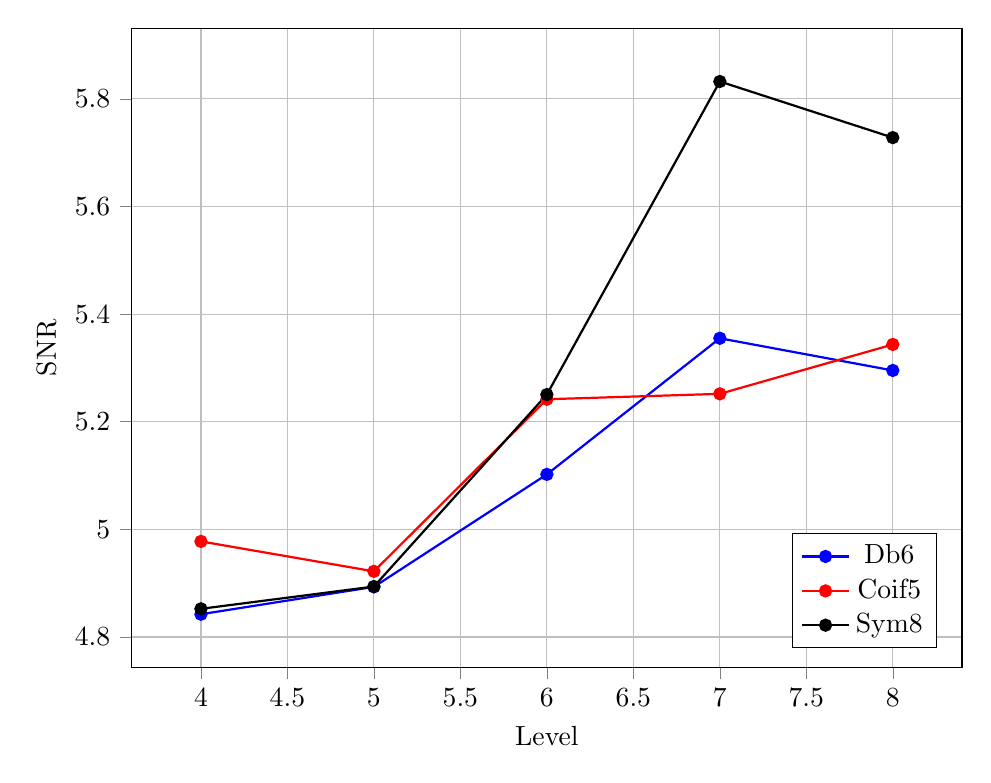
\begin{tikzpicture}
\begin{axis}[
    tick align=outside,
    xtick pos=bottom,ytick pos=left,
    height=0.8\textwidth,
    width=1\textwidth,    
    grid=major,
    % title={Choice of base and levels},
    xlabel={Level},
    ylabel={SNR},
    legend pos=south east,
            ymajorgrids=true,]
\addplot[
    color=blue,
    mark=*,thick, 
    ]
    coordinates {
	(4,4.842219216)
	(5,4.893083055)
	(6,5.102156965)
	(7,5.355110876)
	(8,5.295298758)
    };
\addplot[
    color=red,
    mark=*,thick, 
    ]
    coordinates {    
	(4,4.977584716)
	(5,4.921934414)
	(6,5.241793852)
	(7,5.251832822)
	(8,5.34360019)
    };
\addplot[
    color=black,
    mark=*,thick
    ]
    coordinates {
	(4,4.852302411)
	(5,4.893708271)
	(6,5.250521718)
	(7,5.832332806)
	(8,5.728034433)
    };
\legend{Db6,Coif5,Sym8}
\end{axis}
\end{tikzpicture}
		\caption{Choice of base and levels}
		\label{FIG:wavelet.a}%文中引用该图片代号
	\end{subfigure}\\
	\quad
	\centering
	\begin{subfigure}{1\linewidth}
		\centering
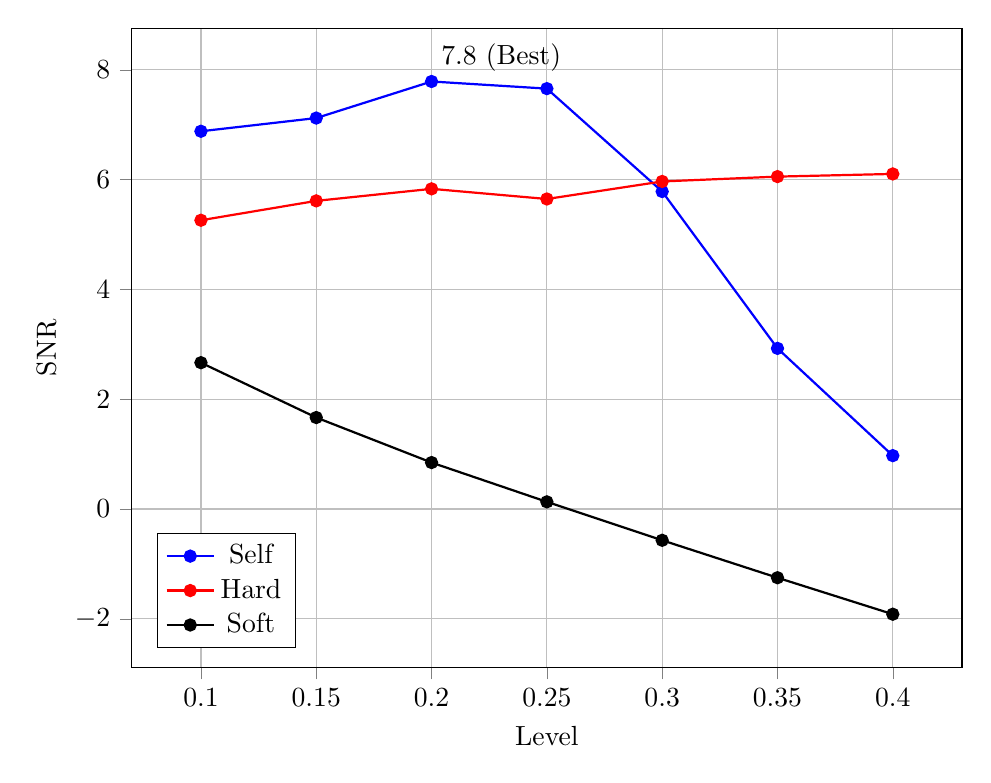
\begin{tikzpicture}
\begin{axis}[
    tick align=outside,
    xtick pos=bottom,ytick pos=left,
    height=0.8\textwidth,
    width=1\textwidth,
    % title={Choice of threshold parameters},
    xlabel={Level},
    ylabel={SNR},
    legend pos=south west,    
    grid=major,
    ymajorgrids=true,]
\addplot[
    color=blue,
    mark=*,thick,
    ]
    coordinates {
(0.1,6.881196846)
(0.15,7.121921467)
(0.2,7.788052276)
(0.25,7.658138472)
(0.3,5.783732988)
(0.35,2.926190942)
(0.4,0.971827728)
    };
\addplot[
    color=red,
    mark=*,thick,
    ]
    coordinates { 
(0.1,5.260228914)
(0.15,5.613376992)
(0.2,5.832332806)
(0.25,5.647585743)
(0.3,5.967033361)
(0.35,6.055329555)
(0.4,6.104046502)
    };
\addplot[
    color=black,
    mark=*,thick,
    ]
    coordinates {
(0.1,2.66541873)
(0.15,1.666208437)
(0.2,0.845928378)
(0.25,0.130262098)
(0.3,-0.570100528)
(0.35,-1.252319888)
(0.4,-1.91680774)
    };
\legend{Self,Hard,Soft}
% Annotation for the point (0.2, 7.718052276)
\node[above right] at (axis cs:0.2,7.788052276) {7.8 (Best)};
\end{axis}
\end{tikzpicture}
		\caption{Choice of threshold parameters}
		\label{FIG:wavelet.b}%文中引用该图片代号
	\end{subfigure}
\caption{\textbf{Wavelet denoising of short signal.} (\textbf{a}) Best: wavelet denoising with sym8 base at 7-layer decomposition. (\textbf{b}) Best: wavelet denoising with 20\% modulo maximum $f_{self}$.}
\label{FIG:wavelet}
\end{figure}
\subsection{Multi-region fusion auscultation}
The quality of models refers to Eq.\ref{eq:Acc}: Accuracy (Acc), Eq.\ref{eq:Se}: Sensitivity (Se),  Eq.\ref{eq:Sp}: Specificity (Sp) and Eq.\ref{eq:F1}: F1-Score.
\begin{equation}
\begin{split}
    Acc= \frac{TP+TN}{TP+FP+TN+FN}
\end{split}
\label{eq:Acc}
\end{equation}
\begin{equation}
\begin{split}
	Se=   \frac{TP}{TP+FN}
\end{split}
\label{eq:Se}
\end{equation}
\begin{equation}
\begin{split}
  Sp=  \frac{TN}{TN+FP}
\end{split}
\label{eq:Sp}
\end{equation}
\begin{equation}
\begin{split}
  F1-Score= 2\times\frac{Se\times Sp}{Se+Sp} 
\end{split}
\label{eq:F1}
\end{equation}
For multi-region fusion auscultation, the average accuracies are 99.35\%, 98.71\%, and 99.14\%, respectively. In terms of average sensitivity, these models achieve 99.08\%, 99.09\%, and 100.00\%, respectively. Furthermore, the average specificity for these models is measured at 99.75\%, 98.10\%, and 97.95\%, respectively. The average F1-Scores are 99.42\%, 98.59\%, and 98.97\%, respectively.

Tab.\ref{tab:HF Diagnosis 10-fold Results} also presents the results obtained from the Yaseen dataset. DenseHF-Net, ResNet-18, and MobileNetV1-28 typically reached convergence around 50 epochs. The AS diagnosis exhibits the best performance, with sensitivity and specificity exceeding 82\% across all three models. For MS and MR, all three models achieve correct diagnoses, with sensitivity and specificity exceeding 87\% in both ResNet-18 and MobileNetV1-28. However, MVP diagnosis by DenseHF-Net yields suboptimal results, with a specificity of only 30\% and an F1-Score of only 45.88\%.

\begin{table*}[htbp]
\centering
\caption{Classification results of HF-Diagnosis dataset and public Yassen Dataset.}
\label{tab:HF Diagnosis 10-fold Results}
\begin{tabular*}{\tblwidth}{LCCLCCLCC}
\toprule
\multicolumn{9}{c}{\textbf{Multi-region fusion auscultation results}} \\
\textbf{DenseHF-Net(ours)}&\multicolumn{2}{c|}{$Average\pm sd$}&ResNet-18&\multicolumn{2}{c|}{$Average\pm sd$}&MobileNetV1-28&\multicolumn{2}{c}{$Average\pm sd$}\\
\hline
$Acc(\%)$&\multicolumn{2}{c|}{$99.35\pm0.71$}&$Acc(\%)$&\multicolumn{2}{c|}{$98.71\pm1.26$}&$Acc(\%)$&\multicolumn{2}{c}{$99.14\pm0.65$}\\
$Se(\%)$&\multicolumn{2}{c|}{$99.08\pm1.22$}&$Se(\%)$&\multicolumn{2}{c|}{$99.09\pm0.92$}&$Se(\%)$&\multicolumn{2}{c}{$100.00\pm0.00$}\\
$Sp(\%)$&\multicolumn{2}{c|}{$99.75\pm0.75$}&$Sp(\%)$&\multicolumn{2}{c|}{$98.10\pm2.68$}&$Sp(\%)$&\multicolumn{2}{c}{$97.95\pm1.54$}\\
$F1-Score(\%)$&\multicolumn{2}{c|}{$99.42\pm0.64$}&$F1-Score(\%)$&\multicolumn{2}{c|}{$98.59\pm1.49$}&$F1-Score(\%)$&\multicolumn{2}{c}{$98.97\pm0.78$}\\
\end{tabular*}
\begin{tabular*}{\tblwidth}{LCCLCCLCC}
        \multicolumn{9}{c}{\textbf{Mitral valve auscultation results}} \\
\textbf{DenseHF-Net(ours)}&\multicolumn{2}{c|}{$Average\pm sd$}&ResNet-18&\multicolumn{2}{c|}{$Average\pm sd$}&MobileNetV1-28&\multicolumn{2}{c}{$Average\pm sd$}\\
\hline
$Acc(\%)$&\multicolumn{2}{c|}{$94.41\pm1.78$}&$Acc(\%)$&\multicolumn{2}{c|}{$91.33\pm2.48$}&$Acc(\%)$&\multicolumn{2}{c}{$90.73\pm1.80$}\\
$Se(\%)$&\multicolumn{2}{c|}{$96.11\pm1.88$}&$Se(\%)$&\multicolumn{2}{c|}{$92.32\pm2.59$}&$Se(\%)$&\multicolumn{2}{c}{$90.68\pm2.49$}\\
$Sp(\%)$&\multicolumn{2}{c|}{$92.00\pm4.08$}&$Sp(\%)$&\multicolumn{2}{c|}{$90.20\pm4.49$}&$Sp(\%)$&\multicolumn{2}{c}{$90.80\pm2.97$}\\
$F1-Score(\%)$&\multicolumn{2}{c|}{$93.95\pm2.15$}&$F1-Score(\%)$&\multicolumn{2}{c|}{$91.17\pm2.58$}&$F1-Score(\%)$&\multicolumn{2}{c}{$90.69\pm1.75$}\\
\end{tabular*}
\begin{tabular*}{\tblwidth}{l|CCCCCCCCCCCC}
        \multicolumn{13}{c}{\textbf{Yaseen dataset results}} \\
        \multicolumn{1}{c}{}&\multicolumn{4}{c}{\textbf{DenseHF-Net(ours)}}&\multicolumn{4}{c}{ResNet-18}& \multicolumn{4}{c}{MobileNetV1-28} \\
        \cmidrule{2-5}\cmidrule{6-9}\cmidrule{10-13}
        \multicolumn{1}{c}{}&AS&MR&MS&MVP&AS&MR&MS&MVP&AS&MR&MS&MVP\\
        \hline
        $Acc(\%)$&91.25&58.75&75.00&63.75&92.50&88.75&95.00&83.75&82.50&92.50&85.00&88.75\\
        $Se(\%)$&	90.00&		97.50&	75.00&	97.50&95.00&	80.00&	90.00&		80.00&	87.50&	87.50&			87.50&	87.50\\
        $Sp(\%)$&	92.50&		20.00&	75.00&	30.00&90.00&	97.50&	100.00&		87.50&	77.50&	97.50&			82.50&	90.00\\
        $F1-Score(\%)$&	91.23&		33.19&	75.00&	45.88&92.43&	87.89&	94.74&		83.58&	82.20&	92.23&			84.93&	88.73\\
        \bottomrule
\end{tabular*}
\end{table*}

\subsection{Mitral valve auscultation}
Fig.\ref{FIG:Average curve} provides a comprehensive overview of the average performance across the mitral valve auscultation dataset. Notably, ResNet-18 and MobileNetV1-28 exhibit comparable performance, while DenseHF-Net exhibits the most rapid rate of improvement. Importantly, all three models exhibit effective convergence of the loss function. It is worth highlighting that both ResNet-18 and MobileNetV1-28 demonstrate similar performance trends, with DenseHF-Net demonstrating the fastest convergence among them.
\begin{figure*}[htbp]
	\centering
	\begin{subfigure}{0.48\linewidth}
		\centering
		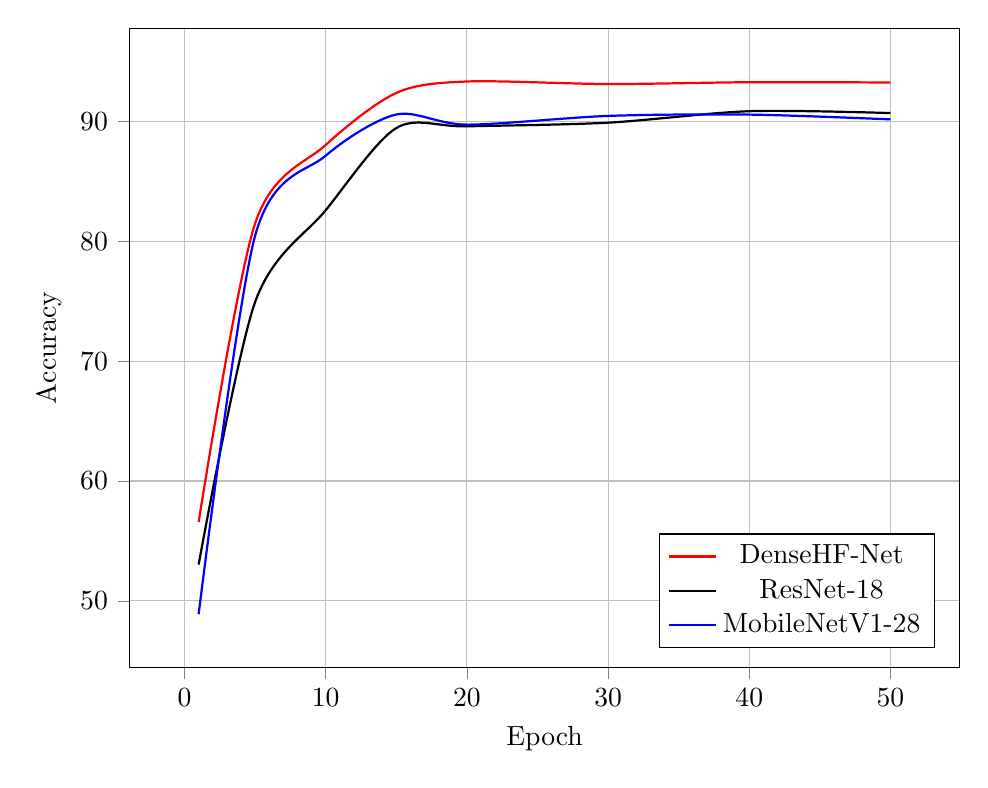
\begin{tikzpicture}
\begin{axis}[
    tick align=outside,
    xtick pos=bottom,ytick pos=left,
    height=0.8\textwidth,
    width=1\textwidth,
    % title={Acc},
    grid=major,
    xlabel={Epoch},
    ylabel={Accuracy},
    xtick={0,10,20,30,40,50},
    ytick={40,50,60,70,80,90,100},
    legend pos=south east,
    ymajorgrids=true,
    % ymajorgrids=true,
    % grid style=dashed,
]
\addplot[
    color=red,
    thick,smooth
    ]
    coordinates {
    (1,56.57439232)
    (5,81.50844994)
    (10,88.05410233)
    (15, 92.39710159301757)
    (20,93.35144958)
    (30,93.14015732)
    (40,93.29104004)
    (50,93.26886444)
    };
\addplot[
    color=black,thick,smooth 
    ]
    coordinates {
    (1,53.03143158)
    (5,74.94425697)
    (10,82.60405884)
    (15, 89.46658782958984)
    (20,89.60950089)
    (30,89.91489792)
    (40,90.87188721)
    (50,90.71563797)
    };
    

\addplot[
    color=blue,
    thick,smooth
    ]
    coordinates {    
    (1,48.88370552)
    (5,80.47420158)
    (10,87.15834885)
    (15, 90.59580764770509)
    (20,89.75154495)
    (30,90.47862091)
    (40,90.58779678)
    (50,90.18920288)
    };

\legend{DenseHF-Net,ResNet-18,MobileNetV1-28}
    
\end{axis}
\end{tikzpicture}
		\caption{Mitral valve auscultation testing accuracy.}
		\label{FIG:Average curve.a}%文中引用该图片代号
	\end{subfigure}
	\begin{subfigure}{0.48\linewidth}
		\centering
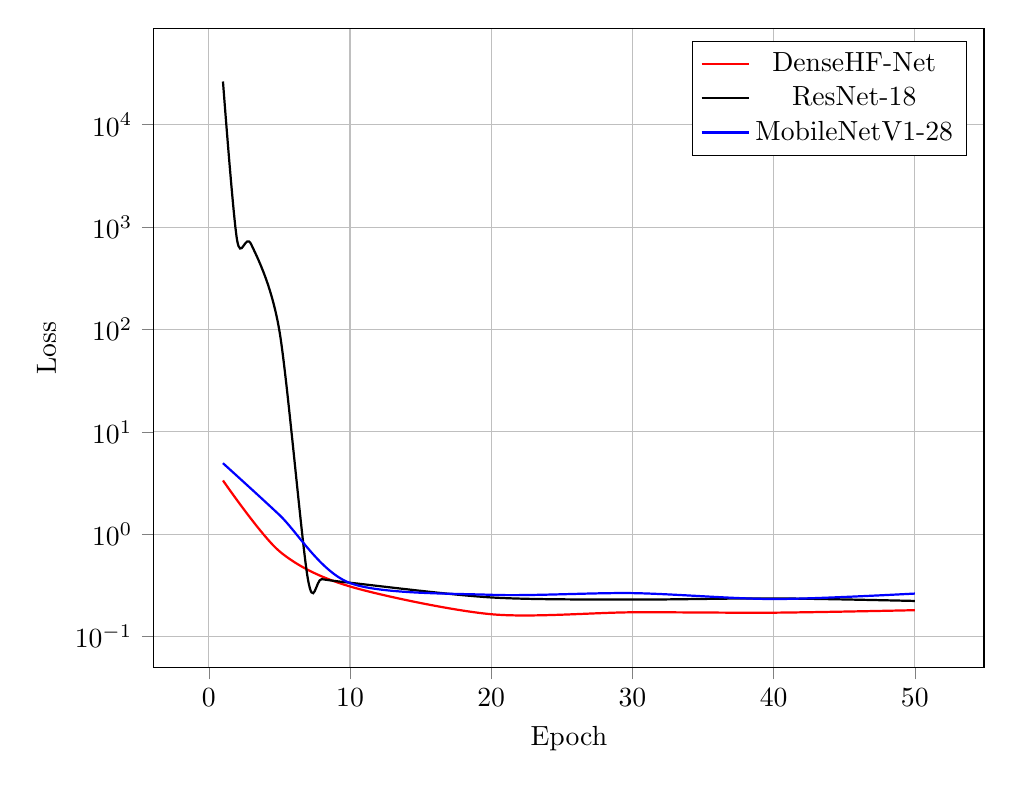
\begin{tikzpicture}
    \begin{axis}[
        tick align=outside,
        xtick pos=bottom,ytick pos=left,
    height=0.8\textwidth,
    width=1\textwidth,
        % title={Acc},
        xlabel=Epoch,
        xtick={0,10,20,30,40,50},
        ytick={0.1,1,10,100,1000,10000},
        ylabel=Loss,
        ymode=log,grid=major,
        log basis y={10},
        ymajorgrids=true,
    % % grid style=dashed,
]
\addplot[
    color=red,thick,smooth
    ]
    coordinates {
    (1,3.355206448)
    (5,0.682259059)
    (10,0.309049669)
    (20,0.165604091)
    (30,0.172943516)
    (40,0.171498471)
    (50,0.18135123)
    };
\addplot[
    color=black,thick,smooth
    ]
    coordinates {
    (1,26451.85823)
    (2,747.1451227188109)
    (3,678.9670787334442)
    (5,96.63756926)
    (7, 0.3756330966949463)
    (8, 0.36473832577466964)
    (10,0.336178899)
    (20,0.241552852)
    (30,0.23027658)
    (40,0.236524488)
    (50,0.223223896)
    };
\addplot[
    color=blue,thick, smooth
    ]
    coordinates {    
    (1,4.946103889)
    (5,1.543885893)
    (10,0.33396288)
    (20,0.25623516)
    (30,0.266215268)
    (40,0.233064194)
    (50,0.263508695)
    };

\legend{DenseHF-Net,ResNet-18,MobileNetV1-28}
    \end{axis}
\end{tikzpicture}
		\caption{Mitral valve auscultation testing loss value.}
		\label{FIG:Average curve.b}%文中引用该图片代号
	\end{subfigure}
\caption{\textbf{Average 10-fold CV history.} (\textbf{a}) Average testing accuracy of three models. (\textbf{b}) Average testing loss of three models (without augmentation).}
\label{FIG:Average curve}
\end{figure*}

Tab.\ref{tab:HF Diagnosis 10-fold Results} lists the 10-fold results of HF diagnosis. DenseHF-Net, ResNet-18, and MobileNetV1-28 basically converge around 50 epochs. 

For mitral valve auscultation, the average accuracies achieved by the individual models are 93.63\%, 91.33\%, and 90.73\%, respectively. In terms of average sensitivity, these models reach 94.28\%, 92.32\%, and 90.68\%, respectively. Furthermore, the average specificity for these models is measured at 92.95\%, 90.20\%, and 90.80\%, respectively. The average F1-Scores for these models are 93.57\%, 91.17\%, and 90.69\%, respectively.

When combined with DenseHF-Net and the ensemble method, the overall performance improves significantly. The resulting average accuracy, sensitivity, specificity, and F1-score are enhanced to 94.41\%, 96.11\%, 92.00\%, and 93.95\%, respectively.
\subsection{Ablation Study}
\subsubsection{Effects of the Model Architecture}
aaaaa
\subsubsection{Effects of Preprocessing and Feature Extraction}
aaa
% \section{Discussion}\label{Discussion}
\subsection{How long should auscultate for?}
The optimal input length for heart sounds in AI models is a subject of debate. Cardiac auscultation offers significant predictive value for cardiac diagnosis, characterized by its rapid and cost-effective nature \cite{taylor2015learning}. In the PhysioNet 2016 dataset, which includes 665 abnormal heart sounds and 2575 normal heart sounds, the lengths of recordings range from 3 seconds to 60 seconds. Meanwhile, the Yaseen dataset consists of 1000 abnormal heart sounds and 200 normal heart sounds, all standardized at a length of 2 seconds.

As illustrated in Fig.\ref{FIG:length}, the choice of input length for heart sounds directly impacts the number of cardiac events included, such as S1, diastole, S2, and systole. Fig.\ref{FIG:length.a} demonstrates that a 1.5-second input can theoretically encompass two diastolic and two systolic events. Fig.\ref{FIG:length.b} shows that a 2-second input can include at least two complete cardiac cycles. Fig.\ref{FIG:length.c} reveals that a 3-second input can accommodate three or four full cardiac cycles. 

For the purposes of this paper, the input length is standardized at 3 seconds.
\begin{figure}[!h]
\centering
    % 插入第一张子图
    \begin{subfigure}{.9\linewidth}
        \centering
        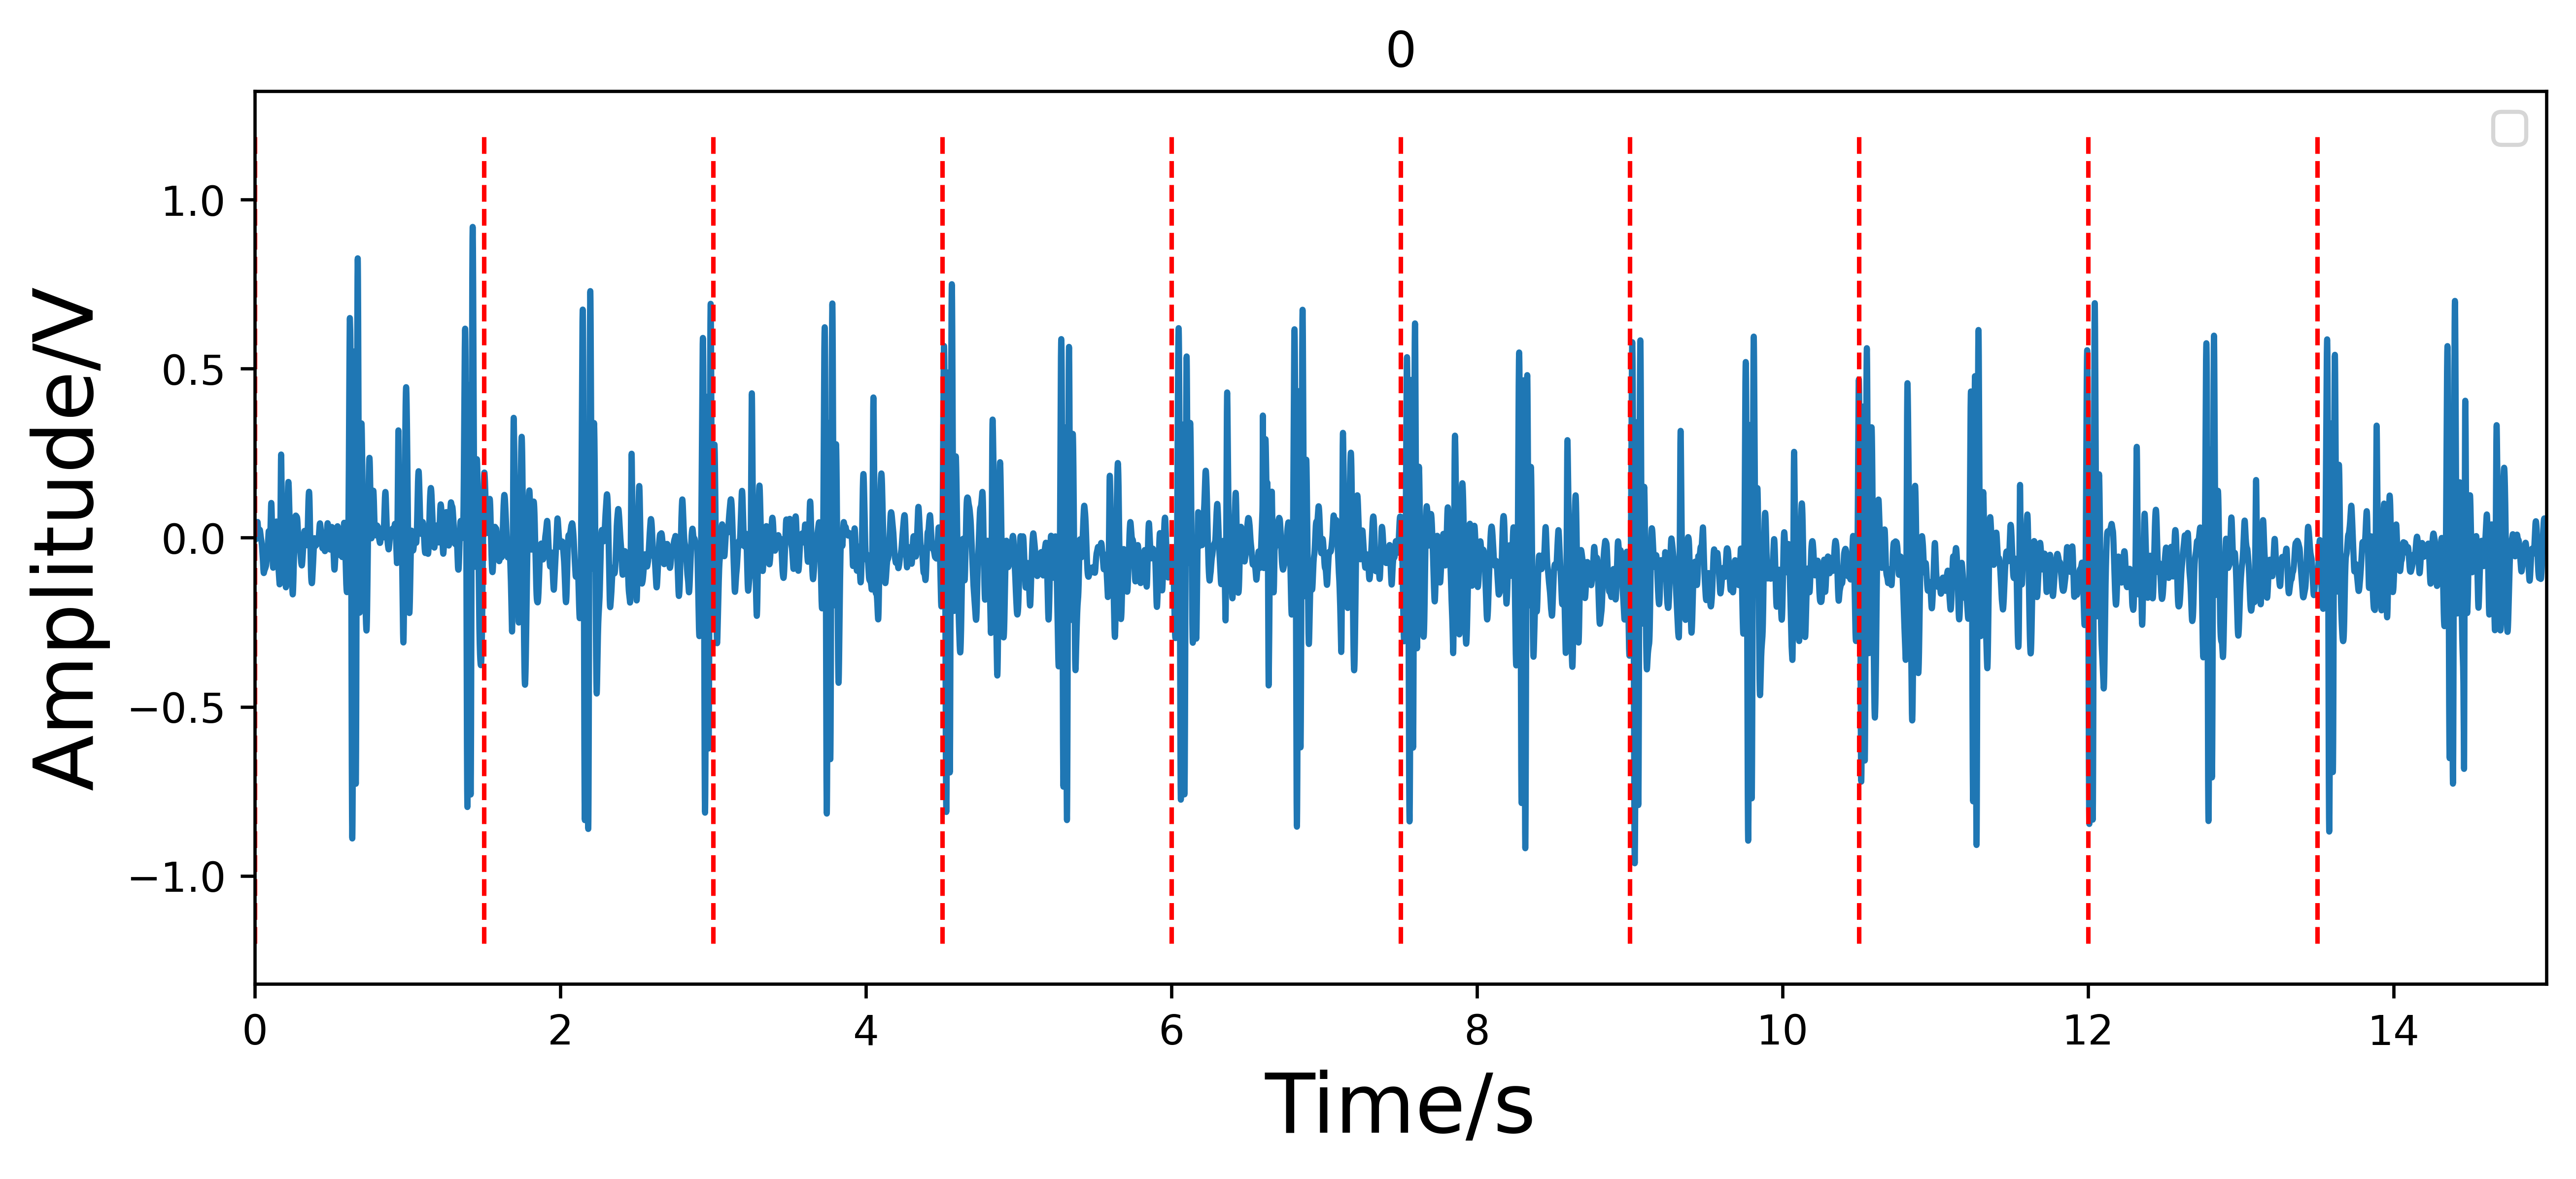
\includegraphics[width=1\linewidth]{figs/disscussion/1.5s.png}
        \caption{Cut with a length of 1.5s}
        \label{FIG:length.a}
    \end{subfigure}\vfill
    % 插入第二张子图
    \begin{subfigure}{.9\linewidth}
        \centering
        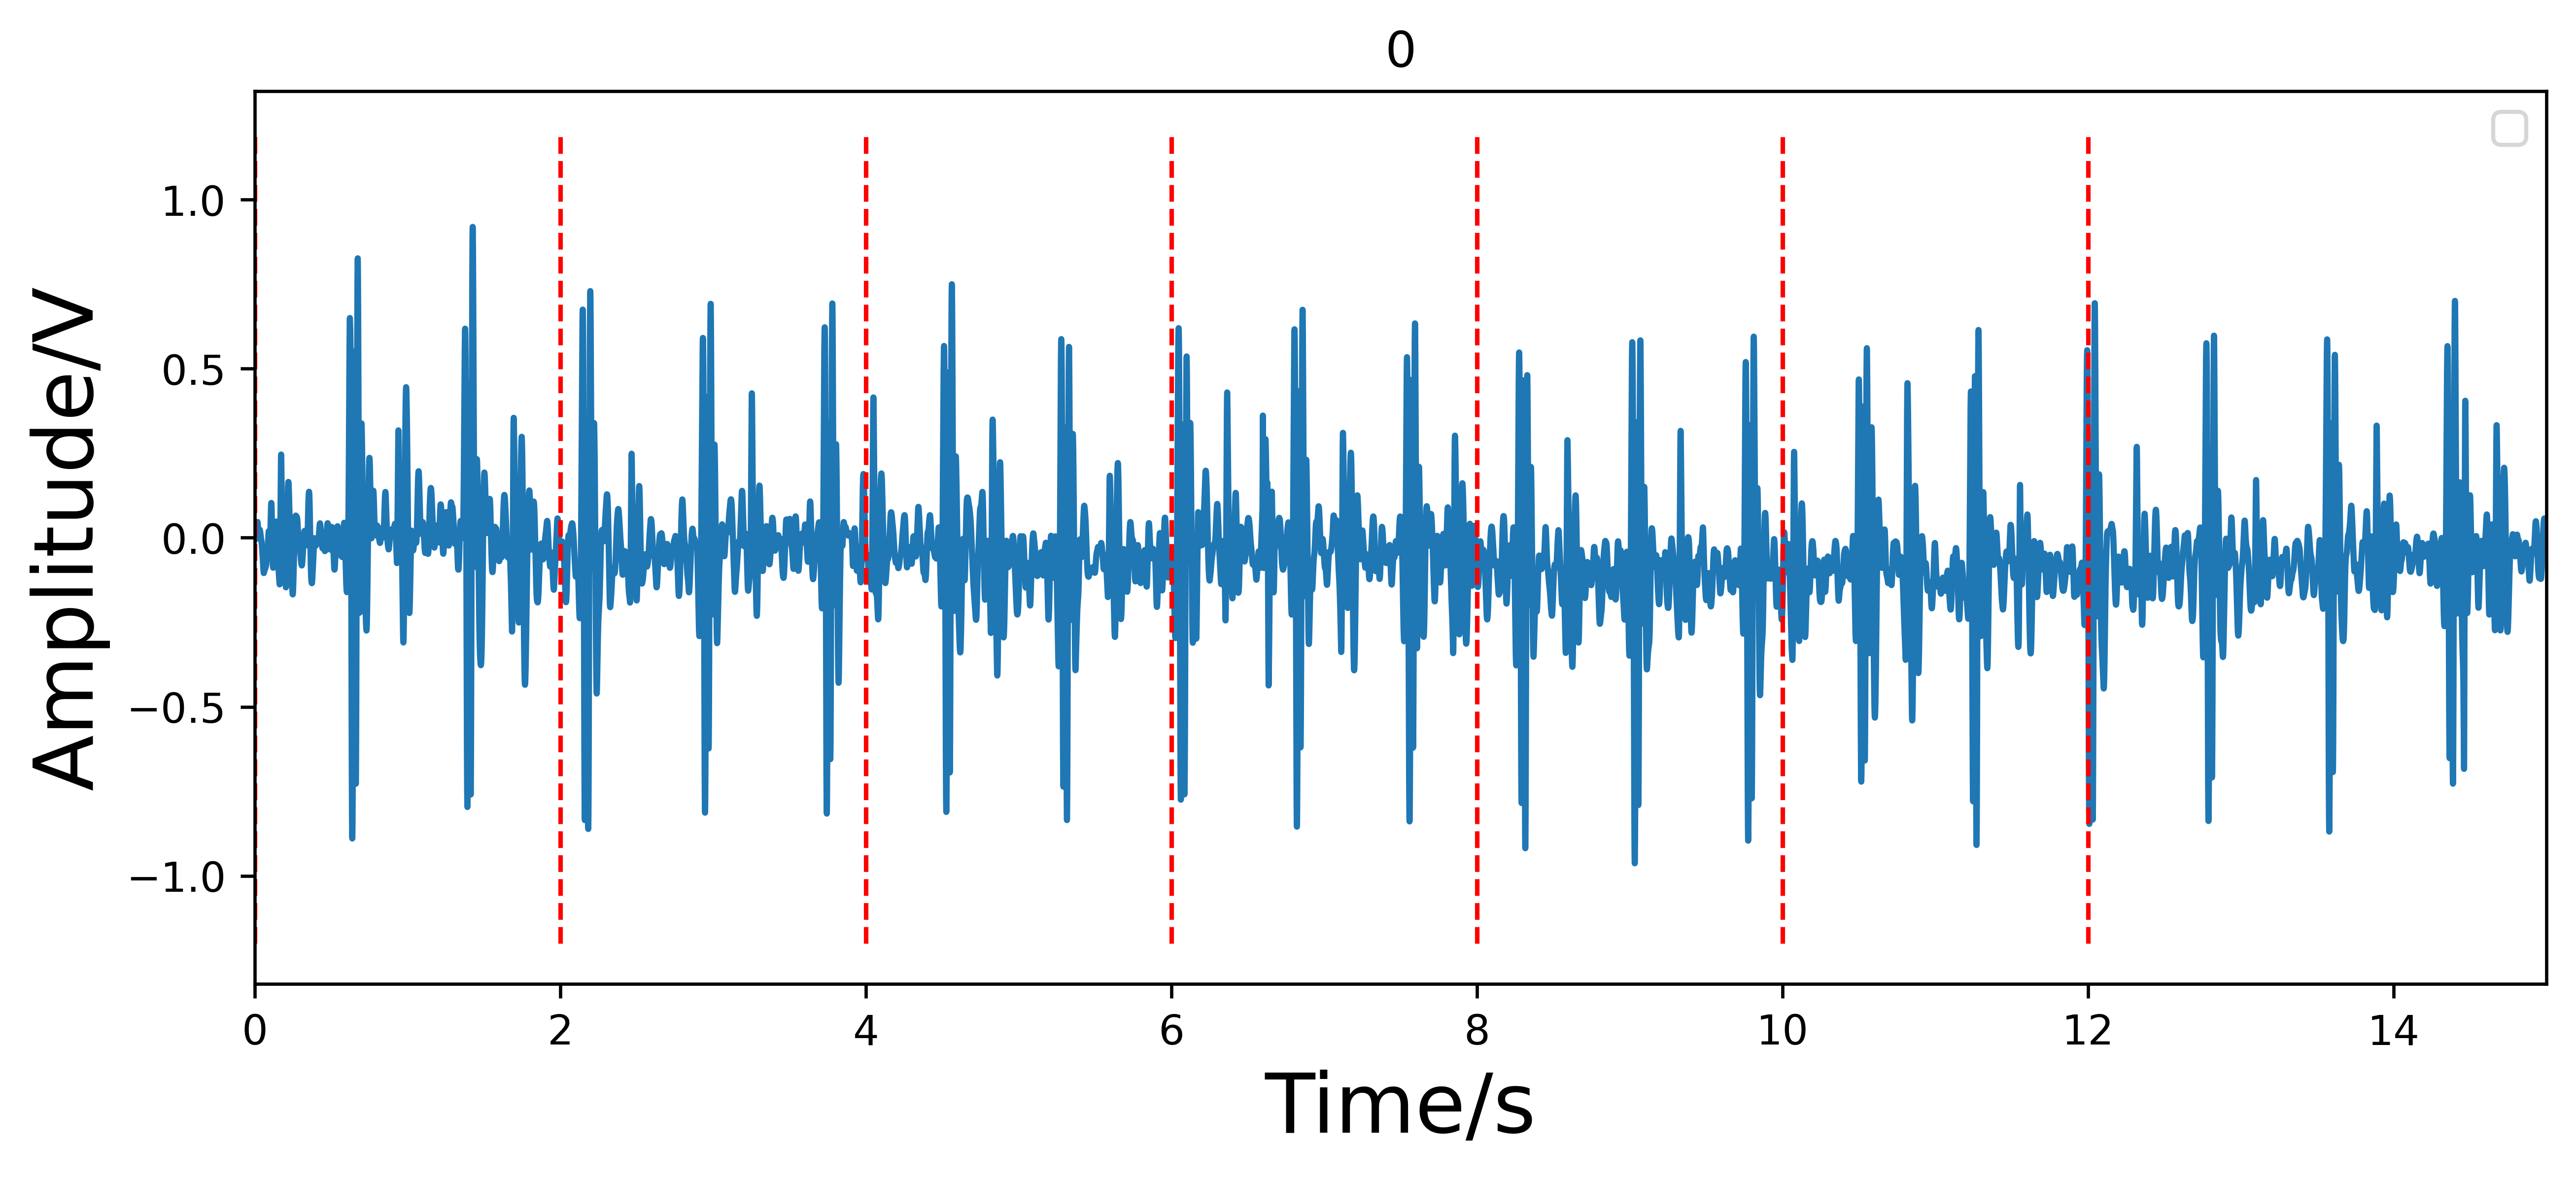
\includegraphics[width=1\linewidth]{figs/disscussion/2s.png}
        \caption{Cut with a length of 2s}
        \label{FIG:length.b}
    \end{subfigure}\vfill
    \begin{subfigure}{.9\linewidth}
        \centering
        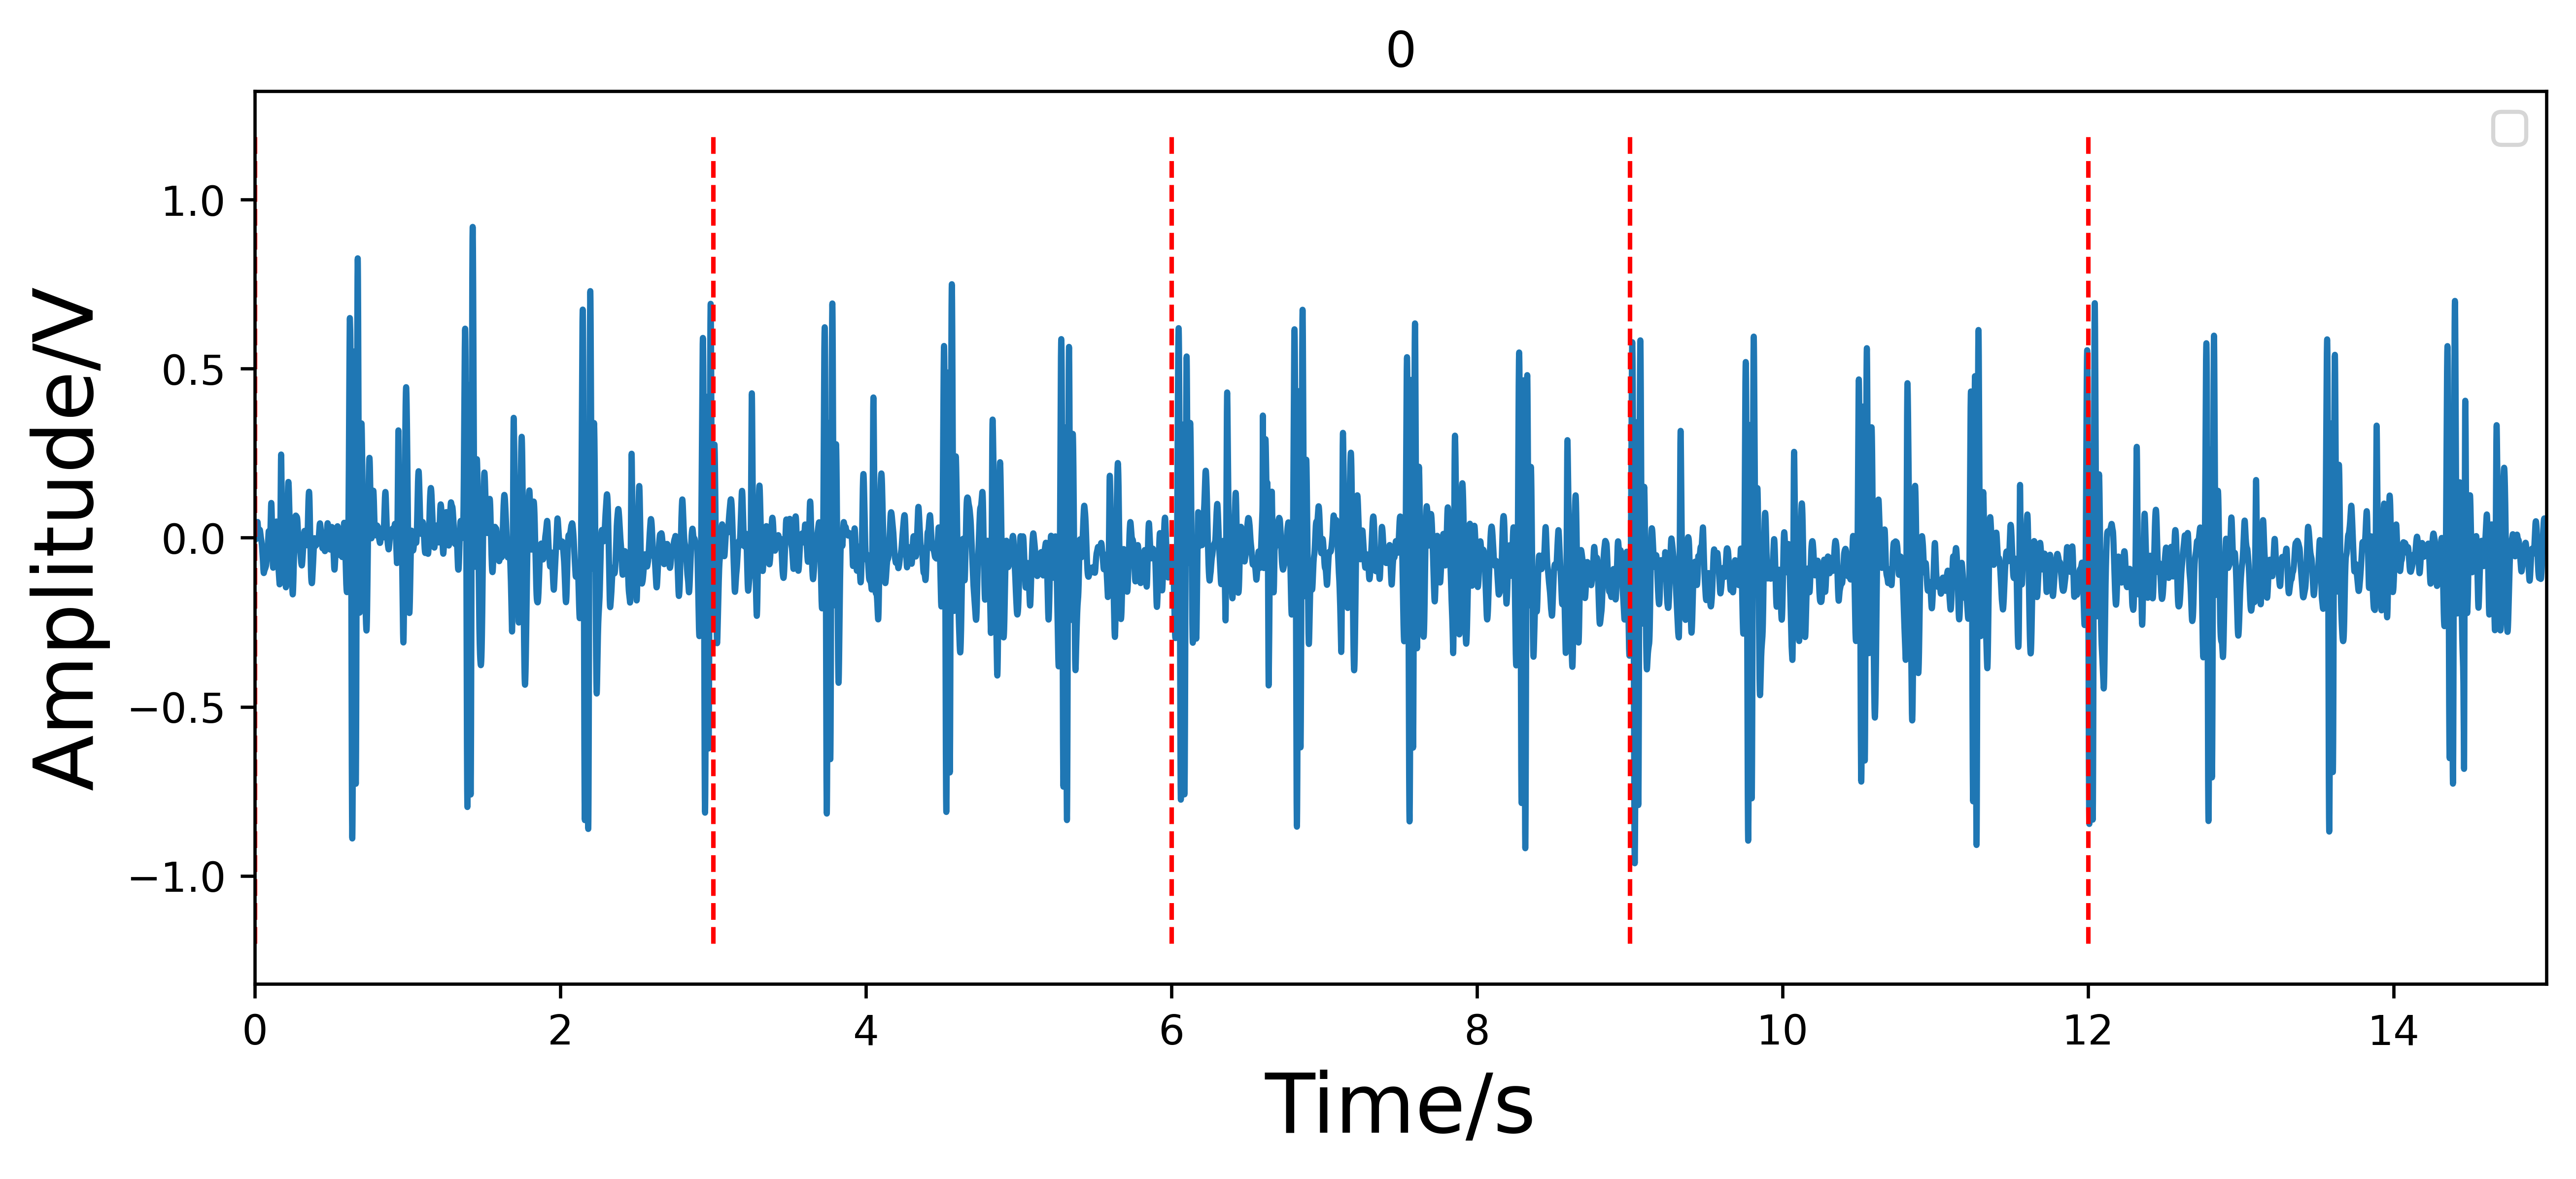
\includegraphics[width=1\linewidth]{figs/disscussion/3s.png}
        \caption{Cut with a length of 3s}
        \label{FIG:length.c}
    \end{subfigure}
\caption{\textbf{Effect of different cutting lengths.} (\textbf{a}) A heart sound is cut with lengths of 1.5s. (\textbf{b}) The same heart sound is cut with lengths of 2s. (\textbf{c}) The same heart sound is cut with lengths of 3s.}
\label{FIG:length}
\end{figure}

\subsection{Interpretability discussion}
Heart sounds contain essential physiological information that reflects the heart's ability to pump blood effectively, and this information is crucial for interpretability in diagnosis. In this study, we analyze the time-frequency characteristics of heart sounds using short-term Fourier transforms (STFT), with a primary focus on the mitral valve, located at the point of the strongest apical beat, to provide a more intuitive explanation.

As illustrated in Fig.\ref{FIG:Time&Frequency.a}, the stable S1 amplitude is predominantly concentrated within the 100 Hz frequency range, clearly reflecting the normal function of the mitral valve. In contrast, the aortic valve, located in the second intercostal space at the right sternal border, is situated further from the heart and is influenced by lung sounds, resulting in a lower signal amplitude. This variation can be explained by the attenuation of energy during sound propagation. The pulmonic valve, positioned in the second intercostal space at the left sternal border, exhibits signal characteristics that are intermediate between those of the mitral and aortic valves, further illustrating the impact of different heart valve locations on heart sound characteristics.

Heart sounds from the mitral valve were collected from the same patient both before and after receiving initial medical intervention, as shown in Fig.\ref{FIG:Time&Frequency.d} and Fig.\ref{FIG:Time&Frequency.e}, providing interpretability of treatment effects. Before treatment, the S1 amplitudes were unstable and were accompanied by noisy lung sounds, indicating impaired heart function. However, after initial treatment, which took place two days later, a noticeable improvement was observed. The heart sound cycle became clearer, and the energy amplitude of S1 was more pronounced, clearly reflecting the positive impact of the treatment on heart function.

\begin{figure*}[h]
\centering
    % 插入第一张子图
    \begin{subfigure}{.3\linewidth}
        \centering
        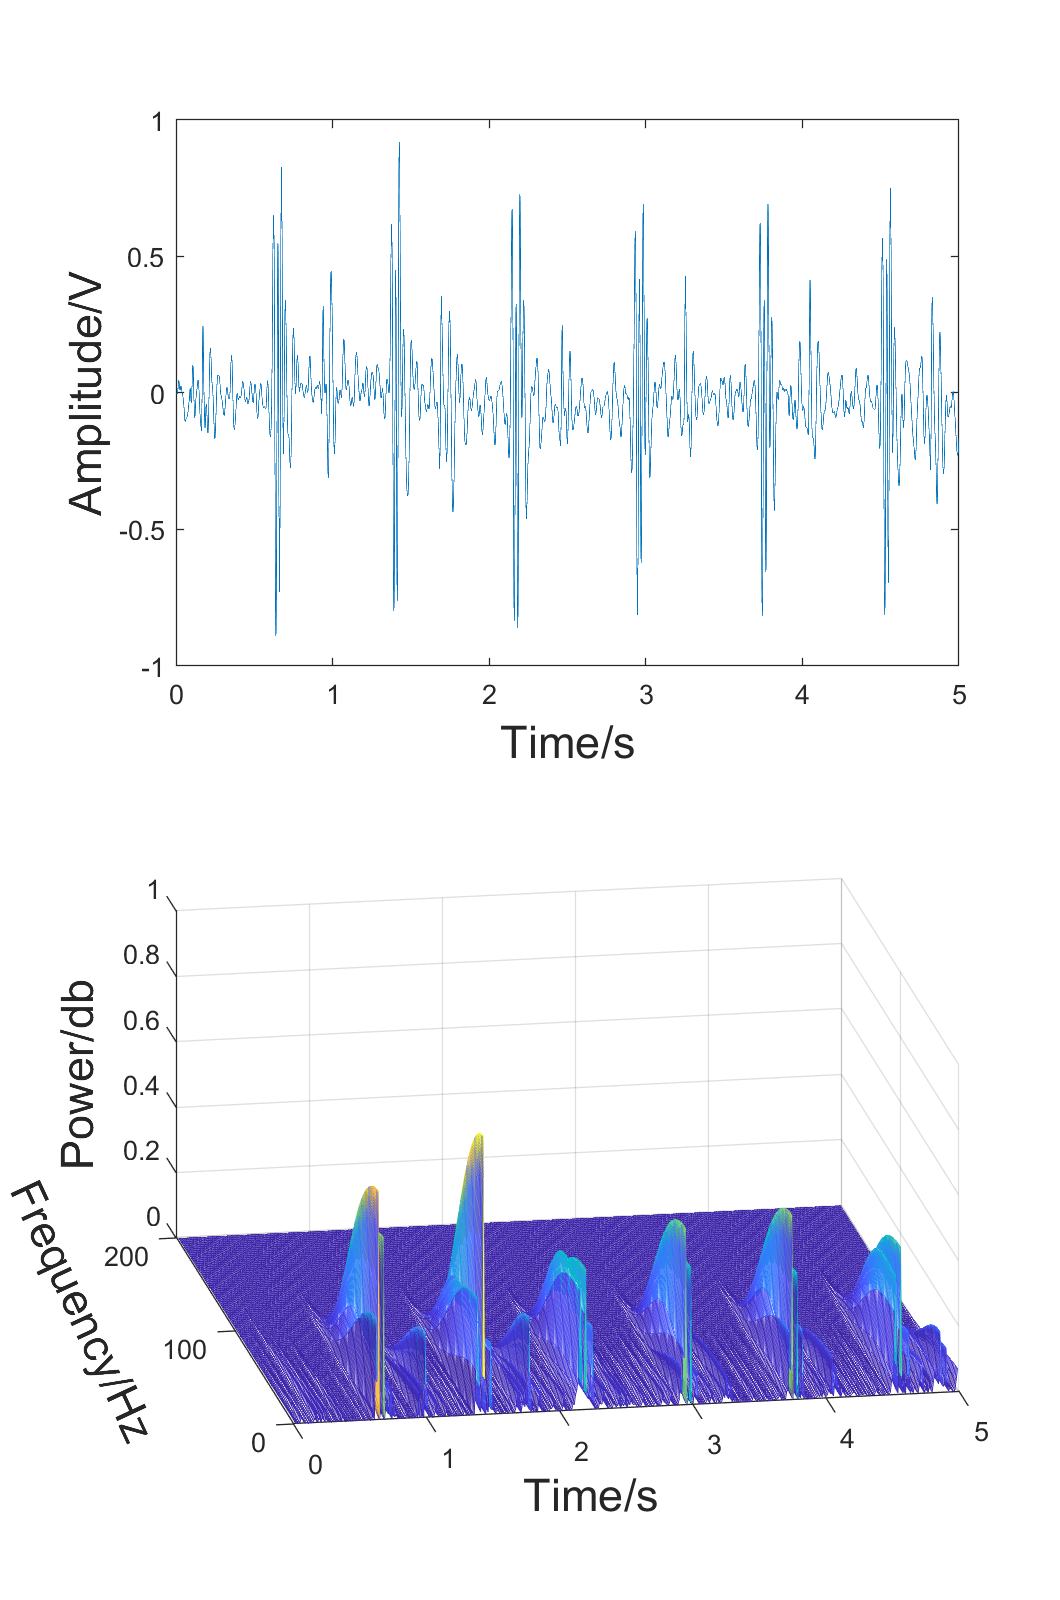
\includegraphics[width=1\linewidth]{figs/disscussion/a.png}
        \caption{Mitral valve}
        \label{FIG:Time&Frequency.a}
    \end{subfigure}\hfill
    % 插入第二张子图
    \begin{subfigure}{.3\linewidth}
        \centering
        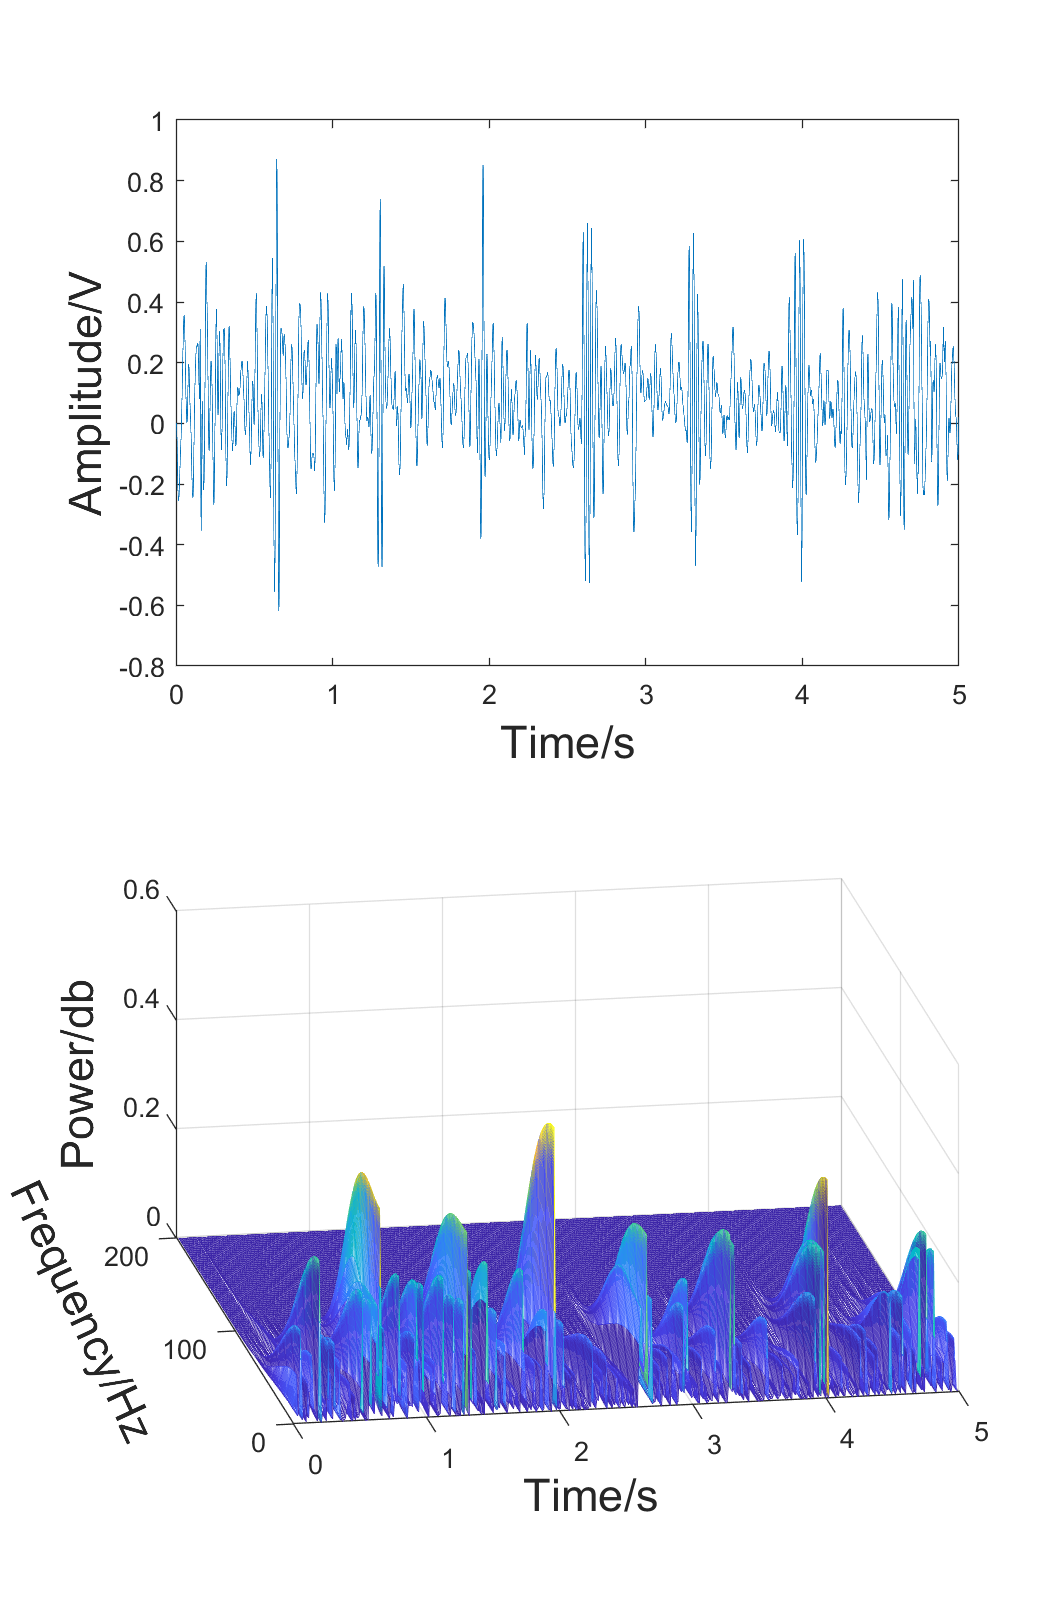
\includegraphics[width=1\linewidth]{figs/disscussion/b.png}
        \caption{Aortic valve}
        \label{FIG:Time&Frequency.b}
    \end{subfigure}\hfill
    \begin{subfigure}{.3\linewidth}
        \centering
        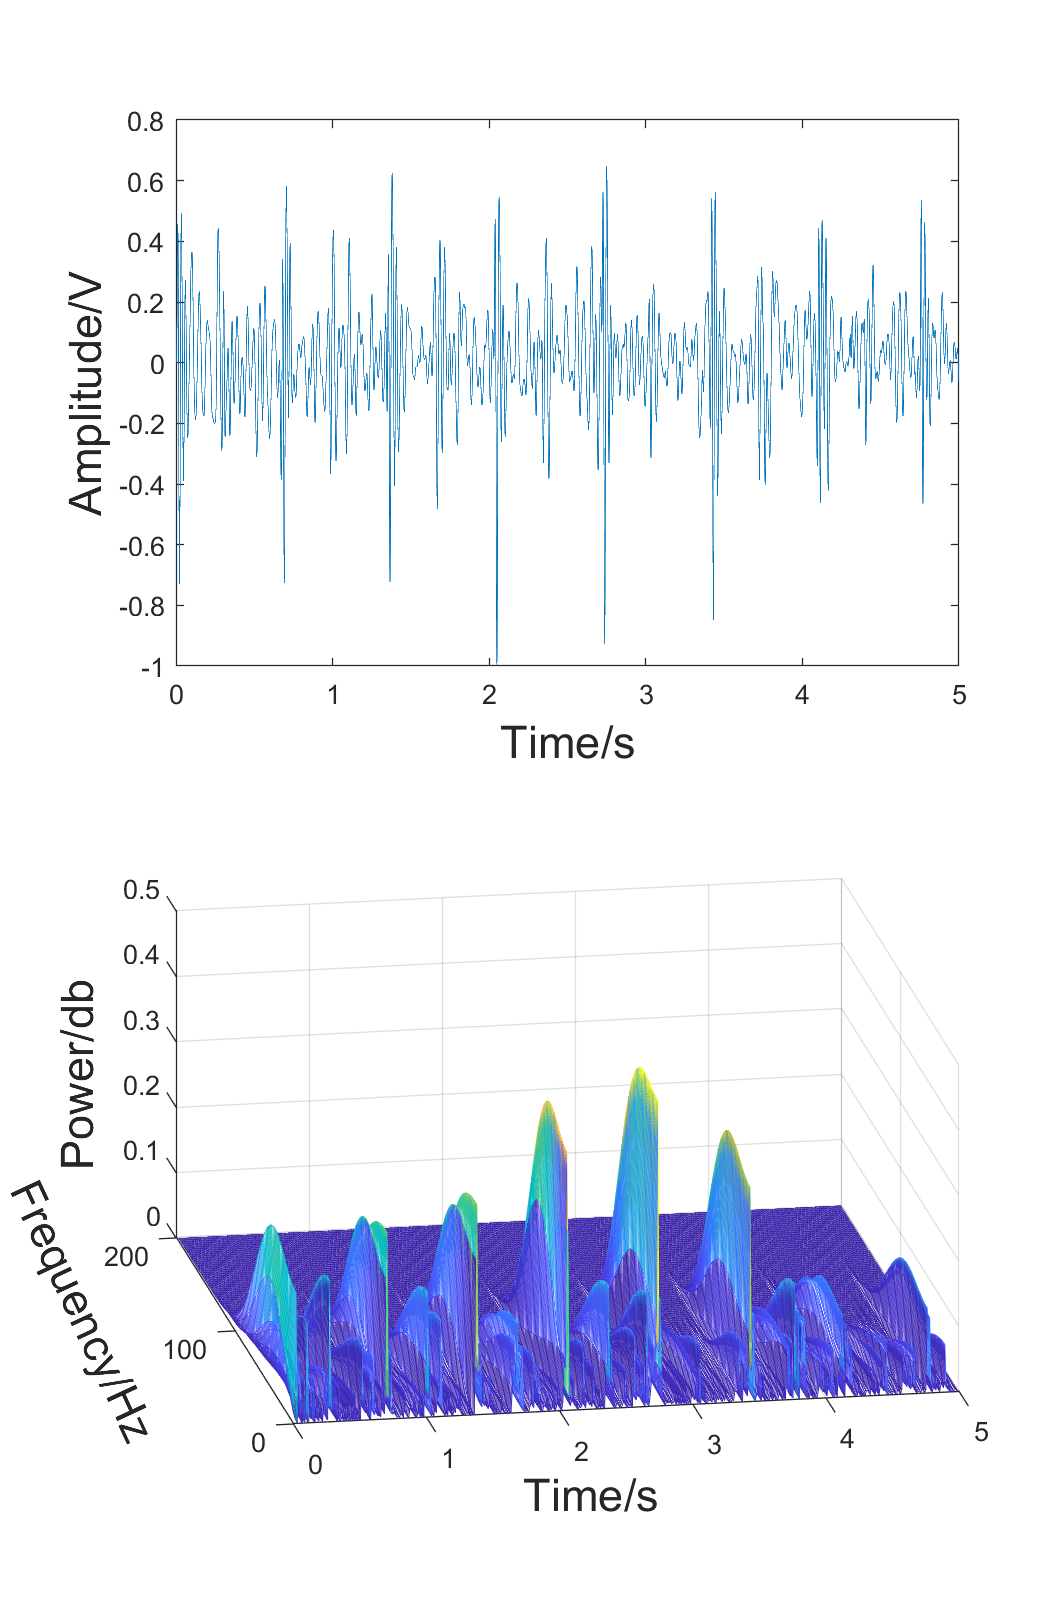
\includegraphics[width=1\linewidth]{figs/disscussion/c.png}
        \caption{Pulmonic valve}
        \label{FIG:Time&Frequency.c}
    \end{subfigure}\\
    \begin{subfigure}{.4\linewidth}
        \centering
        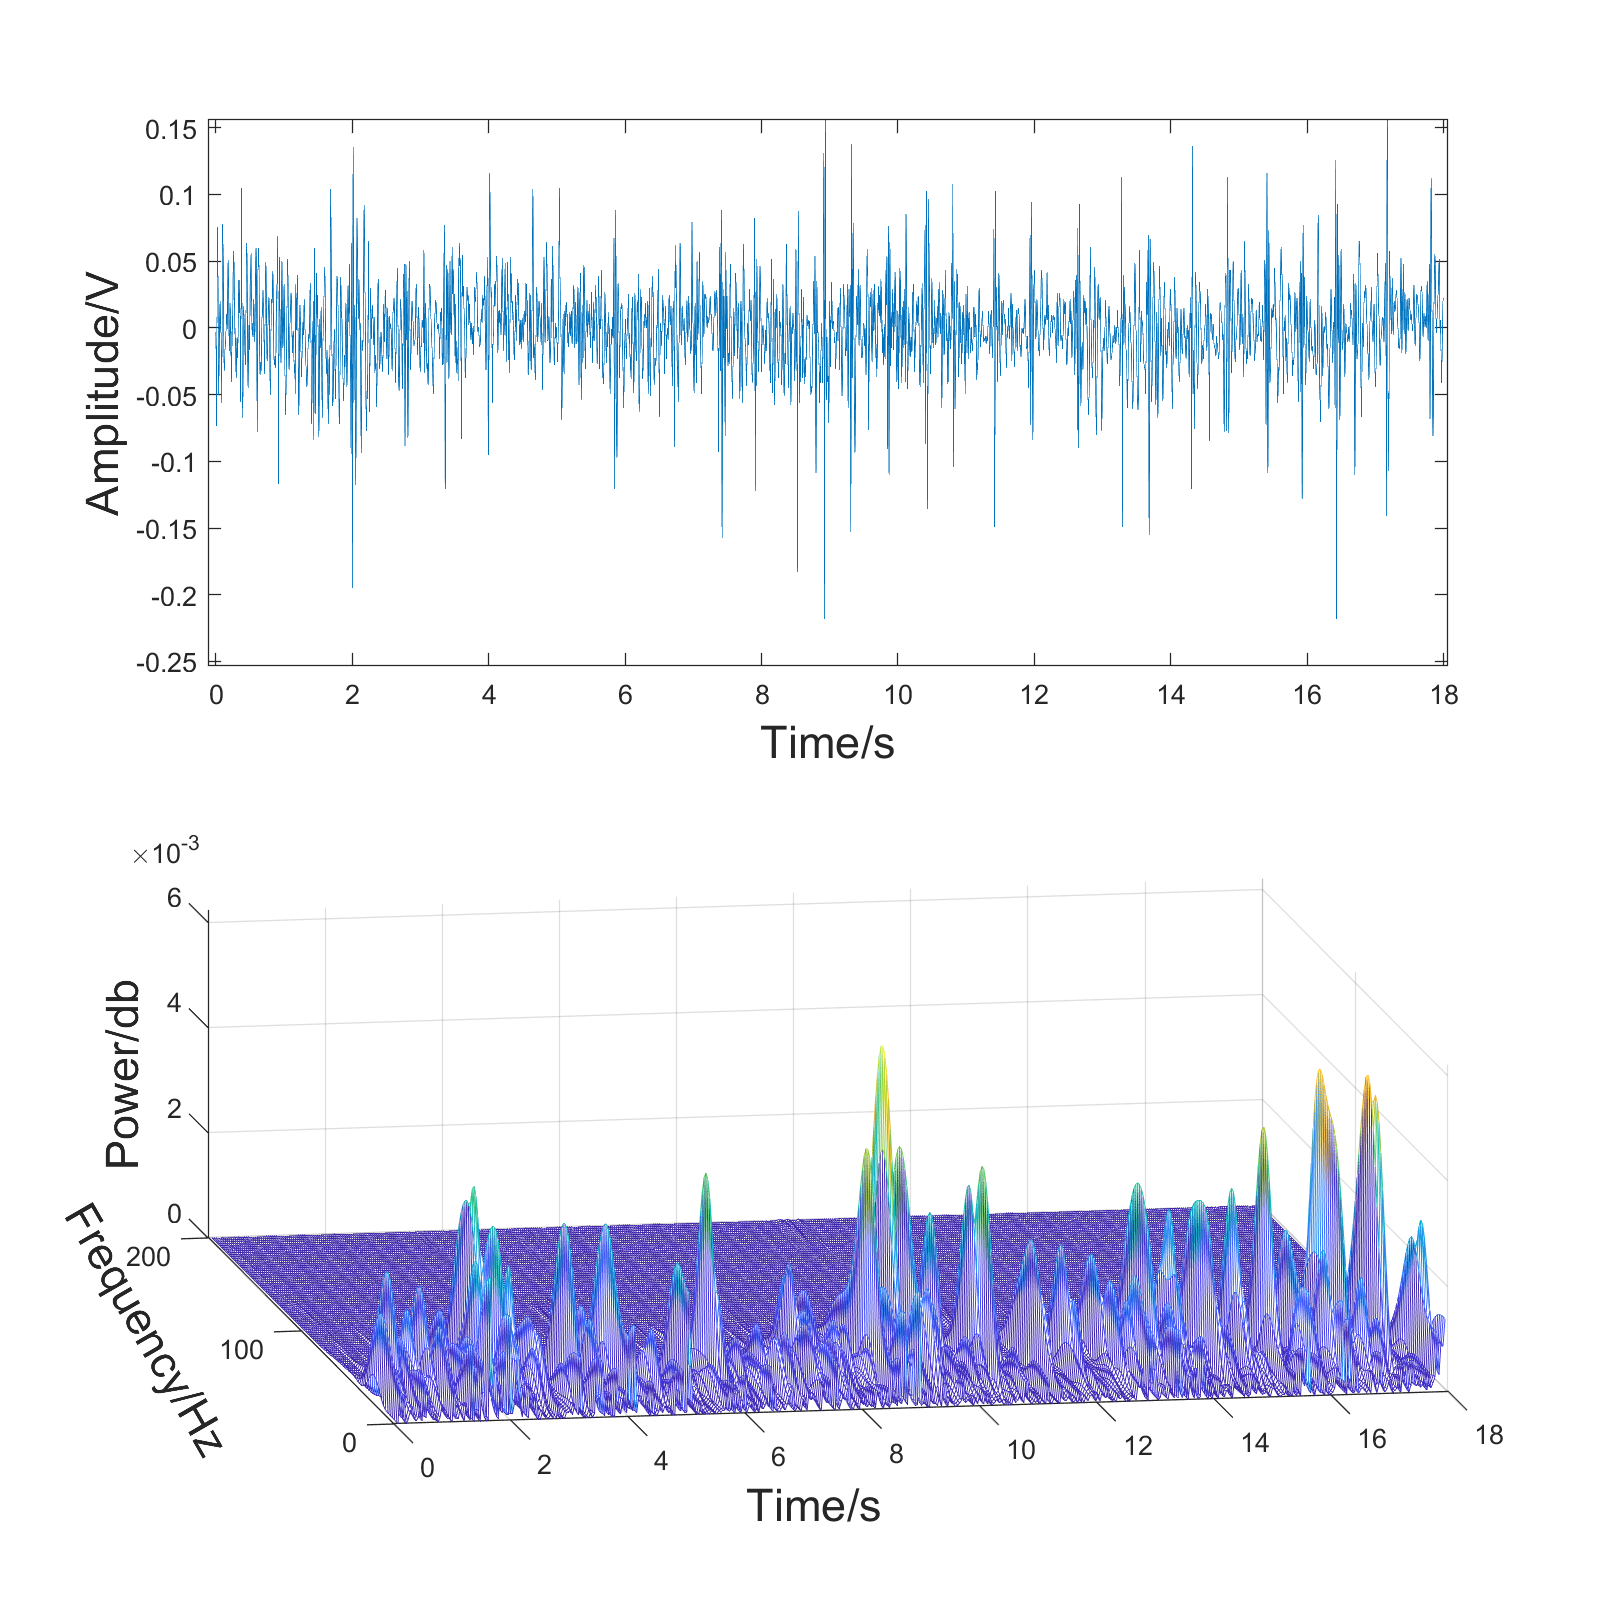
\includegraphics[width=1\linewidth]{figs/disscussion/d.png}
        \caption{Before first-aid}
        \label{FIG:Time&Frequency.d}
    \end{subfigure}\hfill
    % 插入第二张子图
    \begin{subfigure}{.4\linewidth}
        \centering
        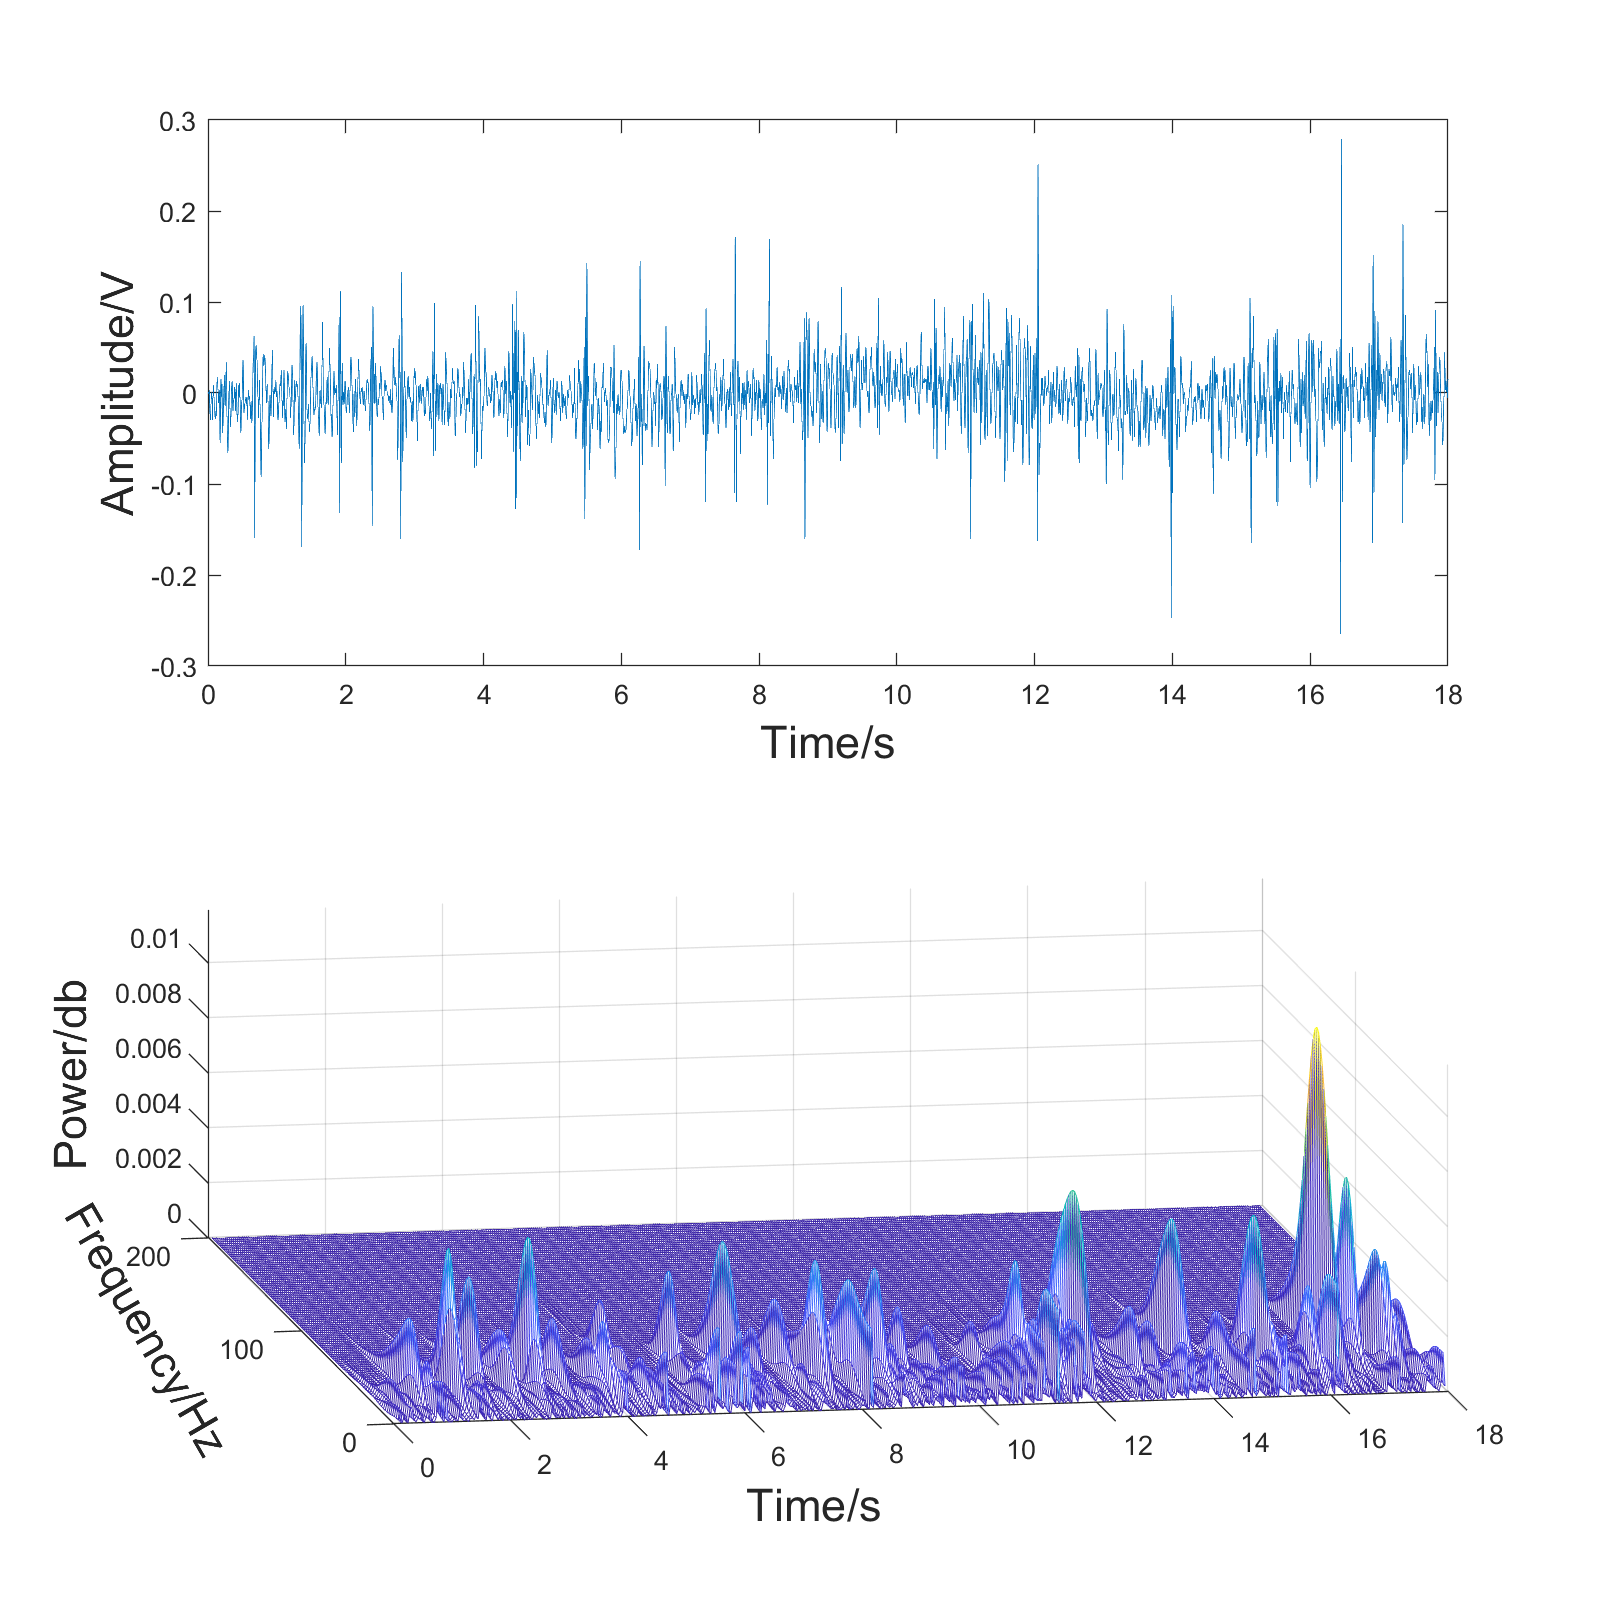
\includegraphics[width=1\linewidth]{figs/disscussion/e.png}
        \caption{After first-aid}
        \label{FIG:Time&Frequency.e}
    \end{subfigure}
\caption{\textbf{Heart sounds in five different situations.} (\textbf{a}) Heart sounds from the mitral valve. (\textbf{b}) Heart sounds from the aortic valve. (\textbf{c}) Heart sounds from the pulmonic valve. (\textbf{d}) Heart sounds before first-aid. (\textbf{e}) Heart sounds after first-aid.}
\label{FIG:Time&Frequency}
\end{figure*}

\subsection{Results discussion}
\subsubsection{Preprocessing and feature extraction}
This paper conducts an in-depth investigation into the optimal decomposition layers, wavelet bases, and threshold shrinkage functions for the denoising of short heart sounds. Fig.\ref{FIG:wavelet} presents our findings, indicating that a 7-layer decomposition using the $f_{self}$ threshold based on the sym8 wavelet yields the most effective denoising results. It's worth noting that Db6 and sym8 wavelets exhibit similar properties, but sym8, due to its shorter support length and superior energy concentration, is more morphologically aligned with heart sounds.

In contrast to previous studies by Chen \cite{2006Research} and Zhao \cite{2010Research}, this paper employs Signal-to-Noise Ratio (SNR) as the primary metric for evaluating noise reduction, avoiding the limitations of waveform comparison. Additionally, our denoising experiments encompass 26 pathological heart sounds, enhancing the clinical relevance of our findings. Furthermore, in comparison to Cheng \cite{cheng2014denoising}, we propose a new $f_{self}$ construction method that significantly improves SNR (7.8 dB).

As depicted in Fig.\ref{FIG:mfcc}, this study delves into the intricacies of feature extraction, particularly focusing on Mel-spectrum and MFCC. The MFCC feature extraction method for heart sounds possesses the advantage of preserving not only temporal waveform features but also capturing frequency energy distribution. This approach retains valuable information aligned with the Mel scale, which corresponds to human auditory perception.

Fig.\ref{FIG:mfcc.a} illustrates a representation of normal heart sounds, while Fig.\ref{FIG:mfcc.b} showcases an instance of heart sounds from a patient with Mitral Valve Prolapse. Both Mel spectrum and MFCC representations encompass a comprehensive range of waveform characteristics, effectively capturing the intricacies of high-frequency signal features in the form of heat maps.
\begin{figure}[!h]
\centering
    % 插入第一张子图
    \begin{subfigure}{.48\linewidth}
        \centering
        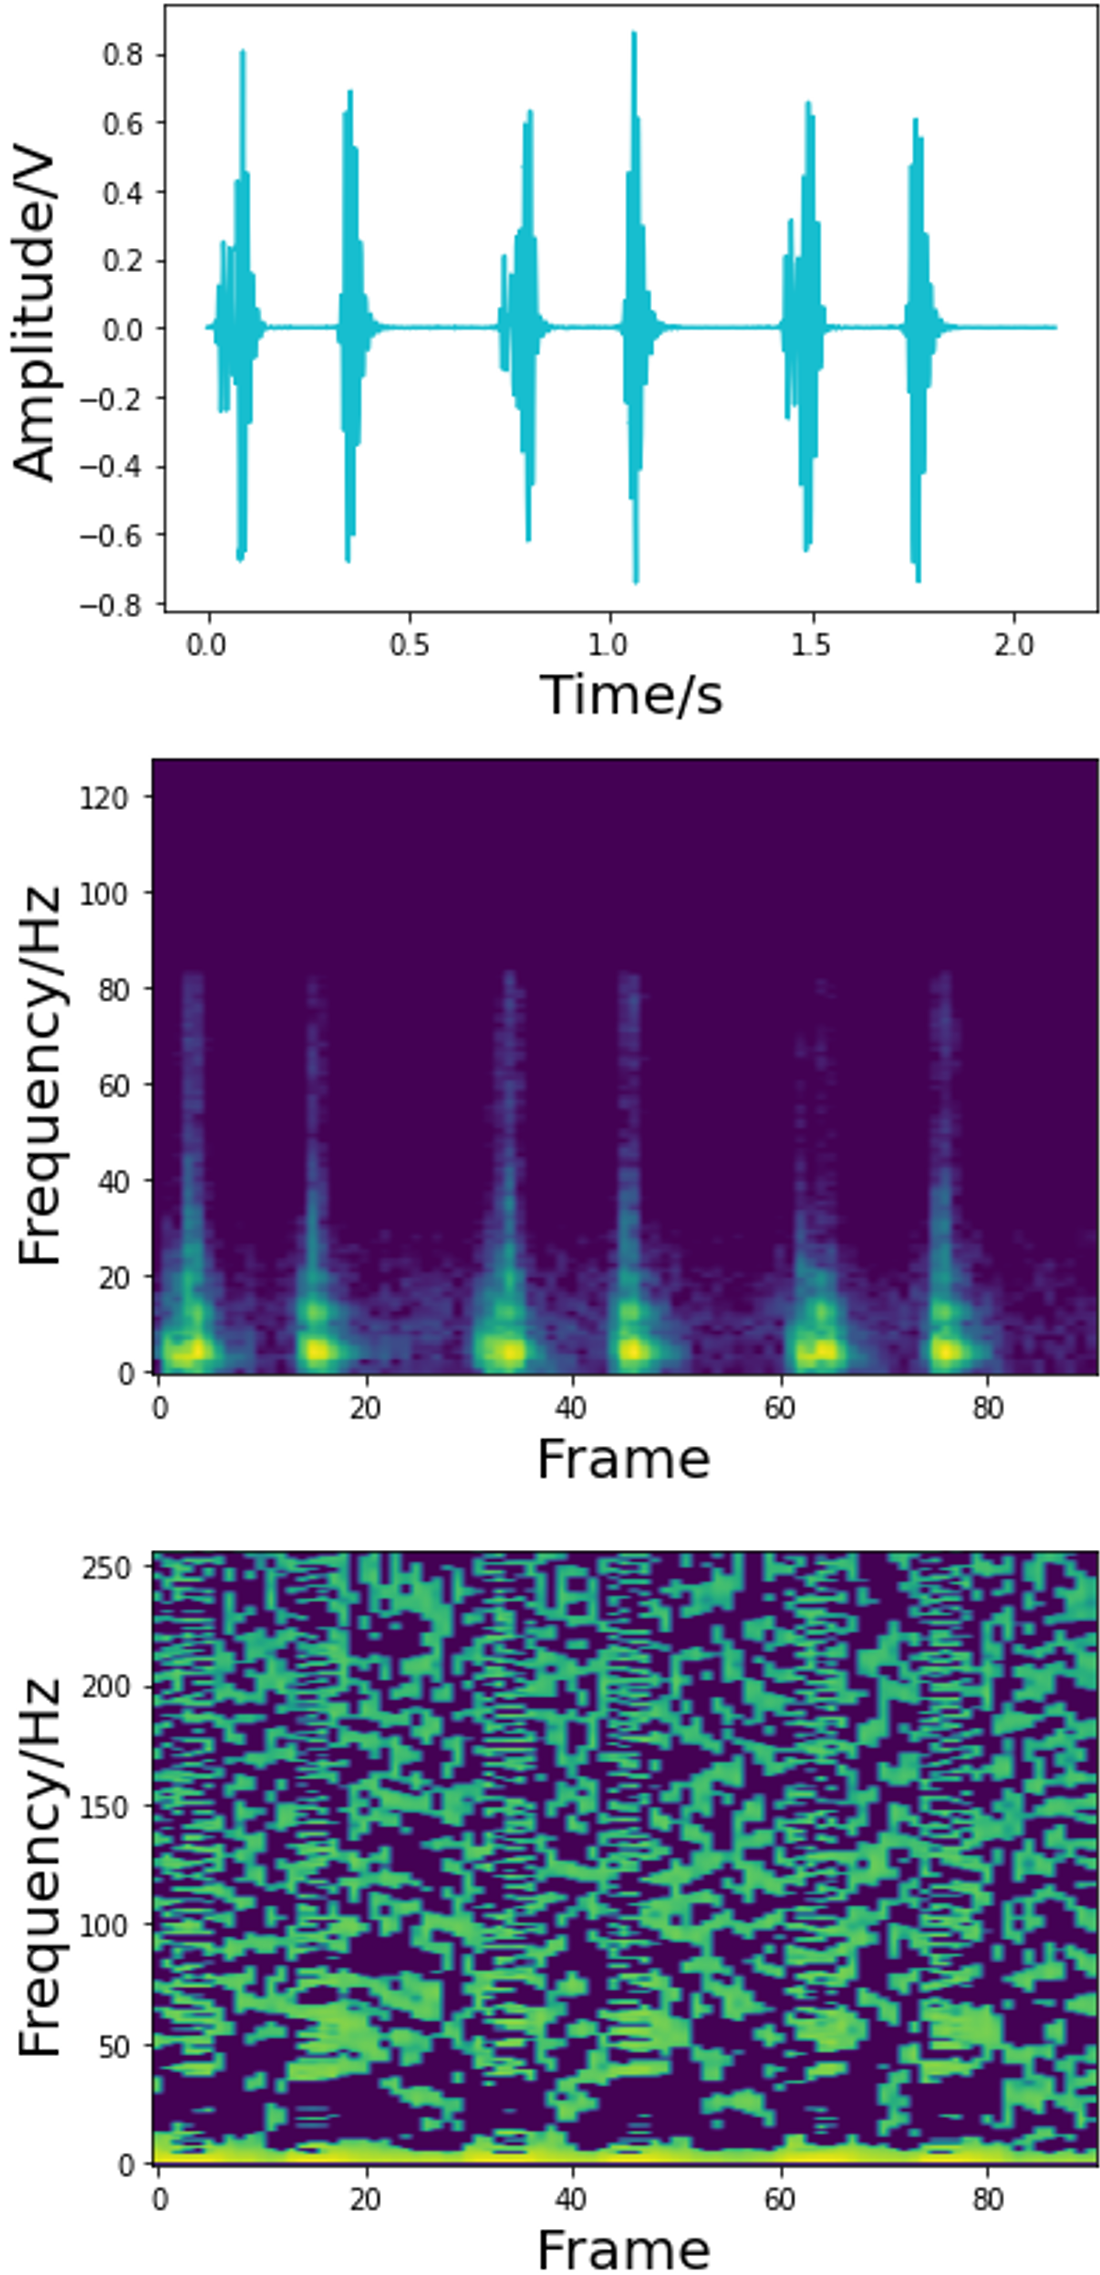
\includegraphics[width=0.99\linewidth]{figs/results/n_mfcc.png}
        \caption{Normal heart sound}
        \label{FIG:mfcc.a}
    \end{subfigure}\hfill
    % 插入第二张子图
    \begin{subfigure}{.48\linewidth}
        \centering
        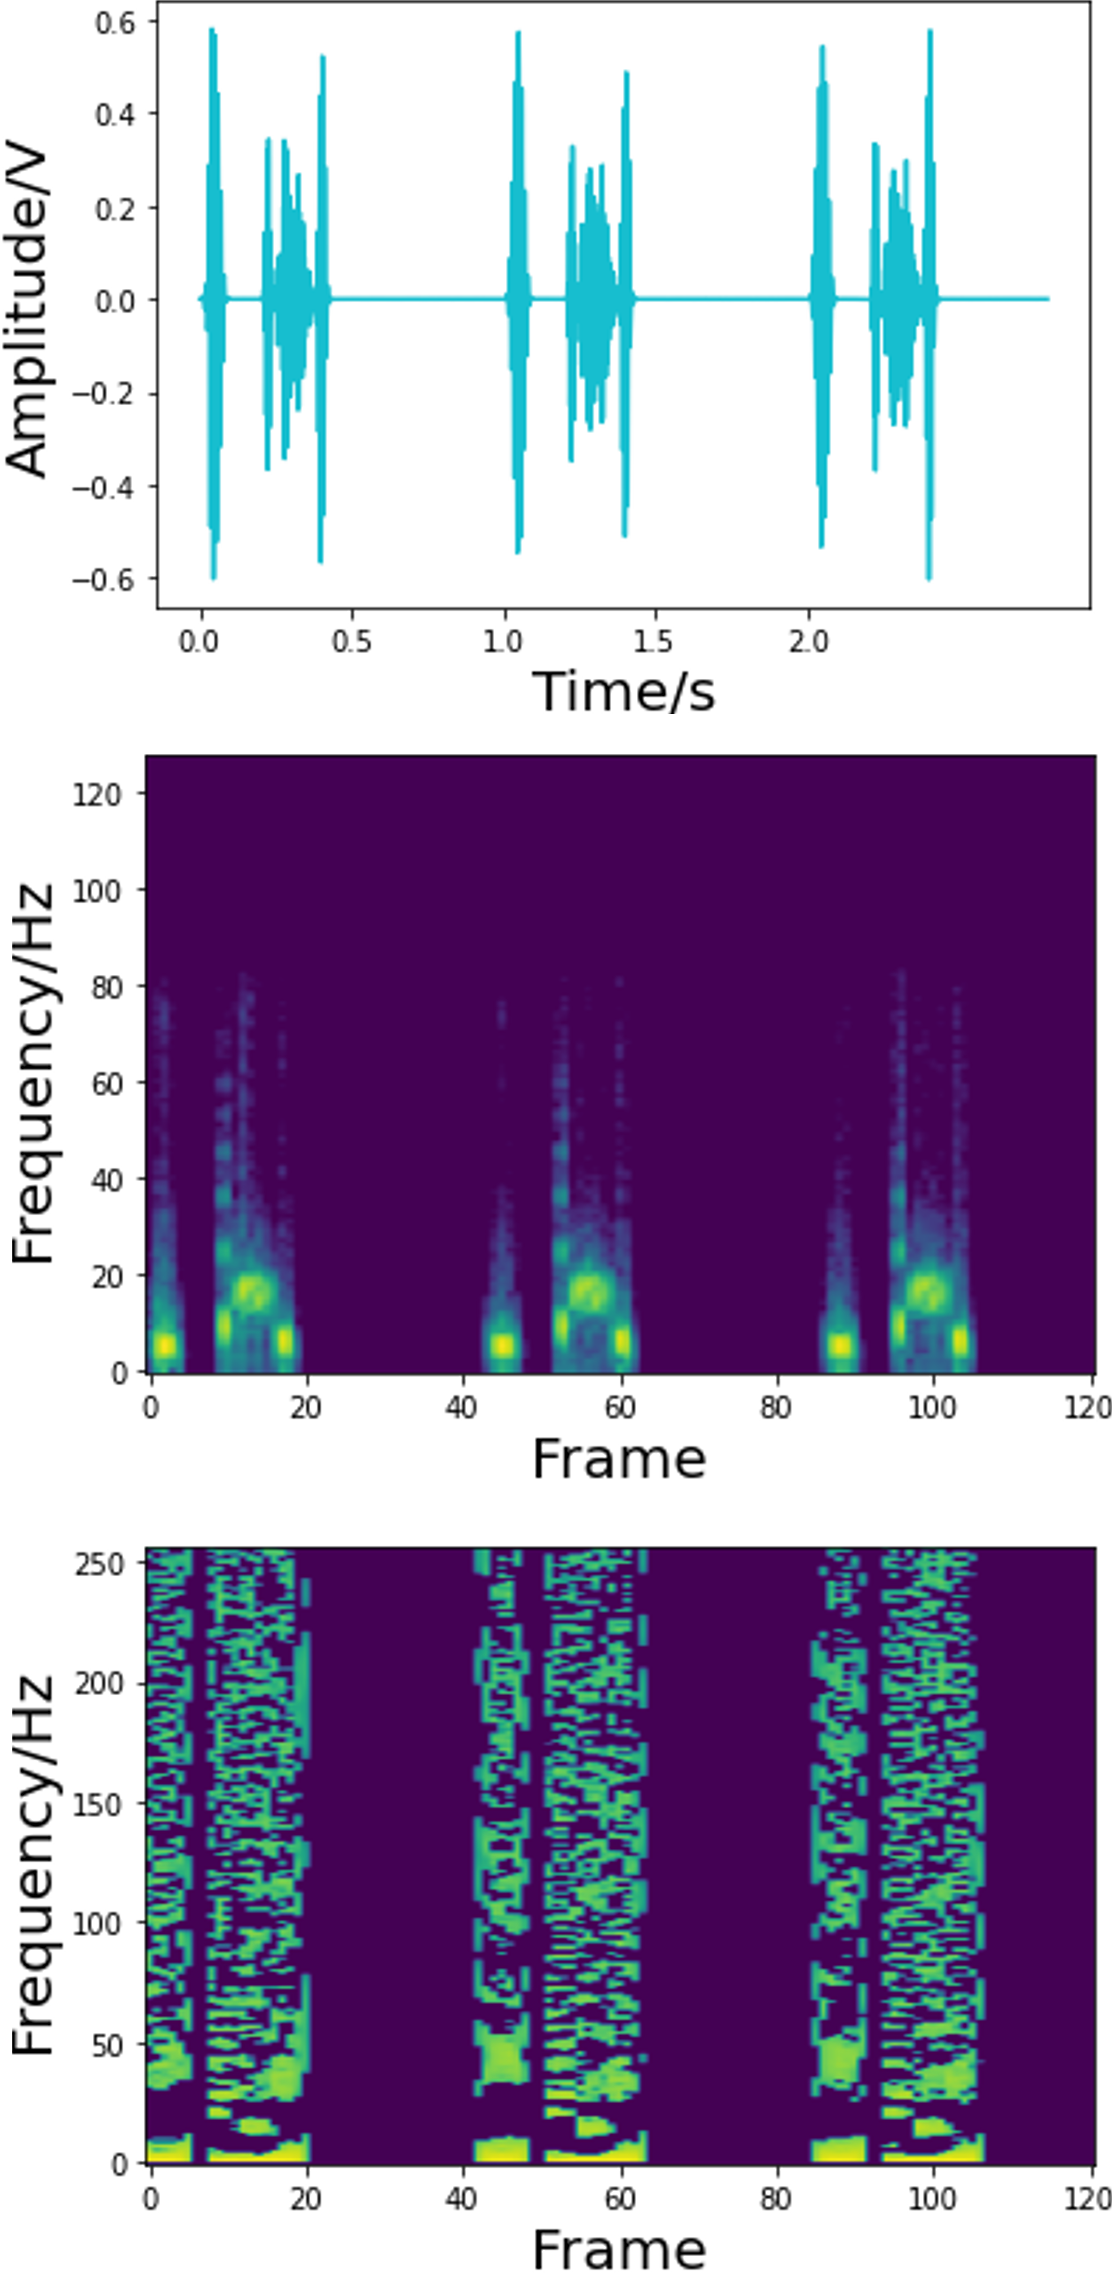
\includegraphics[width=1\linewidth]{figs/results/mvp_mfcc.png}
        \caption{Unhealthy heart sound}
        \label{FIG:mfcc.b}
    \end{subfigure}
\caption{\textbf{Feature extraction result}. (\textbf{a}) Waveform, Mel-spectrum, MFCC of normal heart sound. (\textbf{b}) Waveform, Mel-spectrum, MFCC of unhealthy MVP heart sound.}
\label{FIG:mfcc}
\end{figure}
\subsubsection{Diagnostic performance}
Tab. \ref{tab:HF Diagnosis 10-fold Results} presents the diagnostic outcomes for two heart failure diagnostic datasets and the publicly available Yaseen dataset.

Previous researchers have also explored various intelligent algorithms for heart failure diagnosis or prediction, as shown in Tab. \ref{tab:Comparison}. Khade \cite{khade2019system} and Rao \cite{rao2022explainable} predicted heart failure incidence rates based on physiological parameters or medication records. Acharya \cite{acharya2019deep} and Matsumoto \cite{matsumoto2020diagnosing} examined the potential of diagnosing heart failure using ECG or X-ray images. In comparison to Khade \cite{khade2019system} and Rao \cite{rao2022explainable}, this paper offers enhanced medical diagnostic value and interpretability, along with Acharya \cite{acharya2019deep} and Matsumoto \cite{matsumoto2020diagnosing}. When compared to Acharya \cite{acharya2019deep} and Matsumoto \cite{matsumoto2020diagnosing}, this study theoretically boasts superior diagnostic speed, reduced device size, and more suitable application in ambulance settings.

Compared with previous classification research efforts \cite{vepa2009classification, wu2010hidden, rubin2016classifying, arora2021transfer, li2021lightweight, shuvo2021cardioxnet}, this study incorporates several well-established and successful methods, including wavelet denoising, MFCC feature extraction, and the use of CNNs. We address the issue of signal processing and diagnosis in rapid short-duration auscultation. However, it lacks strong generalization capabilities in diagnosing mitral regurgitation, indicating that the model still suffers from overfitting problems. 
Another limitation is the insufficient discussion of subtypes of AHF.

\begin{table*}[h]
 \caption{Comparison with other researches}
  \label{tab:Comparison}
    \centering
    \begin{tabularx}{\textwidth}{ccccc}
        \toprule
		 \multicolumn{5}{c}{\textbf{Comparison with other heart failure researches}}\\
         \multicolumn{2}{c}{Authors} & \multicolumn{1}{c}{Dataset} & \multicolumn{1}{c}{Aim}& \multicolumn{1}{c}{Acc$(\%)$} \\
        \midrule
        \multicolumn{2}{c}{\textbf{Ours}} & \multicolumn{1}{c}{HF-Diagnosis dataset} & \multicolumn{1}{c}{HF diagnosis}& 94.41\\
        \multicolumn{2}{c}{Khade \cite{khade2019system}} & \multicolumn{1}{c}{Physiological parameters}& \multicolumn{1}{c}{CHF prediction}& 88.30\\
        \multicolumn{2}{c}{Rao \cite{rao2022explainable}} & \multicolumn{1}{c}{Medication records} & \multicolumn{1}{c}{CHF prediction}& 93.00\\
        \multicolumn{2}{c}{Acharya \cite{acharya2019deep}} & \multicolumn{1}{c}{ECG} & \multicolumn{1}{c}{HF diagnosis}& 98.97\\
        \multicolumn{2}{c}{Matsumoto \cite{matsumoto2020diagnosing}} & \multicolumn{1}{c}{X-Ray Images} & \multicolumn{1}{c}{HF diagnosis}  & 82.00\\
        \toprule
		 \multicolumn{5}{c}{\textbf{Comparison with other heart sound researches}}\\
        Authors & Feature extraction & Classification method & Databases & Acc$(\%)$ \\
                \midrule
        \textbf{Ours} & MFCC & DenseHF-Net & Mitral valve auscultation dataset & 94.41 \\
        Vepa \cite{vepa2009classification} & STFT, DWT & kNN, MLP, SVM & Normal, systolic, diastolic records& 95.2\\
        Wu \cite{wu2010hidden} & MFCC & HMM & 325 cycles of 10-type& 95.08 \\
        Rubin \cite{rubin2016classifying} & MFCC & CNN & PhysioNet 2016& 95.2\\
        Arora \cite{arora2021transfer} & STFT & CNN & PhysioNet 2016& 89.04\\
        Li \cite{li2021lightweight} & STFT & CNN & PhysioNet 2016 & 85\\
        Shuvo \cite{shuvo2021cardioxnet} & Time-invariant features &CNN & Yaseen database& 99.6\\
        \bottomrule
    \end{tabularx}
\end{table*}
% \section{Conclusion}\label{Conclusion}
Cardiac auscultation is a crucial clinical method for detecting heart failure and holds significant promise for rapid heart failure detection. This paper discusses signal processing and diagnostic model techniques for the rapid diagnosis of AHF. The average SNR of heart sounds reached 7.8 dB. The models successfully achieve effective feature learning and effective loss convergence. DenseHF-Net stands out as the top-performing model in heart failure diagnosis, achieving an accuracy of 92.60\%. Both auscultation strategies can meet the requirements for emergency vehicles and hospital rooms. Future research will focus on collecting multi-center AHF data for model training, aiming to achieve better generalization performance. Simultaneously, we will actively promote clinical testing and assessment to validate its practicality and explore its clinical emergency application value, ultimately aiming to develop a device similar to that in \cite{2022Audicor} that could obtain FDA approval. Additionally, future research directions will also include expanding the diagnosis to multiple cardiac diseases to further enhance the model's potential in cardiovascular disease detection.
% \section{Data and code availability}\label{Data and code availability}
Data collection has been approved by the medical ethics committee of Tianjin 4th Center Hospital of China (No. 2022-T050). The data used in this study is available at \href{https://github.com/qiuzhaoyu/AHF-Rapid-Diagnosis/Database}{https://github.com/qiuzhaoyu/AHF-Rapid-Diagnosis/Database}. The code used in this study is available at \href{https://github.com/qiuzhaoyu/AHF-Rapid-Diagnosis}{https://github.com/qiuzhaoyu/AHF-Rapid-Diagnosis}.
% \section{Funding}\label{Funding}
This research was supported by The National Natural Science Foundation of China (No. 72174138).
% The authors declare that they have no known competing financial interests or personal relationships that could have appeared to influence the work reported in this paper.
\newpage
% Loading bibliography style file
\bibliographystyle{model1-num-names}
% Loading bibliography database
\bibliography{References.bib}
\end{document}

